\documentclass[10pt,twocolumn,letterpaper]{article}

\usepackage{cvpr}
\usepackage{times}
\usepackage{epsfig}
\usepackage{graphicx}
\usepackage{amsmath}
\usepackage{amssymb}
\usepackage{caption}
\usepackage{verbatim}
\usepackage{subcaption}
\usepackage{algorithm2e}
\usepackage{rotating}
\usepackage[space]{grffile}
\usepackage[font=small,skip=0pt]{caption}
%\DeclareMathOperator{\Tr}{Tr}
% Include other packages here, before hyperref.

% If you comment hyperref and then uncomment it, you should delete
% egpaper.aux before re-running latex.  (Or just hit 'q' on the first latex
% run, let it finish, and you should be clear).
\usepackage[breaklinks=true,bookmarks=false]{hyperref}
\graphicspath{ {figures/} }
% \cvprfinalcopy % *** Uncomment this line for the final submission

\def\cvprPaperID{****} % *** Enter the CVPR Paper ID here
\def\httilde{\mbox{\tt\raisebox{-.5ex}{\symbol{126}}}}

% custom commands
\newcommand{\scream}[1]{{\color{red} \bf *** #1 ***}}

% Pages are numbered in submission mode, and unnumbered in camera-ready
%\ifcvprfinal\pagestyle{empty}\fi
\setcounter{page}{1}
\begin{document}

%%%%%%%%% TITLE
\title{Enriching Object Detection with 2D-3D Registration and Continuous Viewpoint}
%\title{Enrich Object Detection : 2D-3D registration and continuous viewpoint estimation}

\author{First Author\\
Institution1\\
Institution1 address\\
{\tt\small firstauthor@i1.org}
% For a paper whose authors are all at the same institution,
% omit the following lines up until the closing ``}''.
% Additional authors and addresses can be added with ``\and'',
% just like the second author.
% To save space, use either the email address or home page, not both
\and
Second Author\\
Institution2\\
First line of institution2 address\\
{\tt\small secondauthor@i2.org}
}

\maketitle
%\thispagestyle{empty}

%%%%%%%%% ABSTRACT
\begin{abstract}
A large body of recent work on object detection has focused on exploiting 3D CAD model databases to improve detection performance. Many of these approaches work by aligning exact 3D models to images using templates generated from renderings of the 3D models at a finite set of discrete viewpoints. The training procedures for these approaches, however, are very expensive and require gigabytes of memory and storage, and the viewpoint discretization hampers pose estimation performance.

We propose an efficient method for synthesizing templates from 3D models that runs on the fly -- that is, it quickly produces detectors for an arbitrary viewpoint of a 3D model without expensive dataset-dependent training or template storage. Given a 3D model and an arbitrary continuous detection viewpoint, our method synthesizes a discriminative template by extracting features from a rendered view of the object and decorrelating spatial dependences among the features. Our decorrelation procedure relies on a gradient-based algorithm that is more numerically stable than standard decomposition-based procedures, and we efficiently search for candidate detections by computing FFT-based template convolutions. Due to the speed of our template synthesis procedure, we are able to perform joint optimization on continuous scale, translation, rotation, and focal length. We provide an efficient GPU implementation of our algorithm, and we validate its performance on 3DObject dataset and PASCAL 2012 dataset.

%     Using 3D model to detect and register the model to RGB image has been a growing field of study. Recently, Aubry \etal \cite{Aubry14} and J. Lim \etal \cite{Lim14} tried to estimate pose and align exact CAD model to an image using part-based templates. Malisiewicz \etal \cite{Malisiewicz11} also addresses the issue by transferring metadata after detection. Hejrati \etal \cite{Hejrati14} uses template synthesis to detect an object. All these approaches require extensive training, a lot of memory space. Also, the training based approach requires defining fixed viewpoints which limit themselves.
%  To overcome these difficulties, we propose an efficient and fast way to synthesize and validate templates using on the fly realistic rendering that can jointly optimize scale, translation, rotation and focal length continuously. We render an object and extract features and decorrelate spatial dependencies within them on the fly to make a discriminative template. To speed up the decorrelation procedure, we adopt a gradient based algorithm which is numerically more stable than decomposition procedure. Finally, we efficiently search for candidate match by computing convolution using FFT and jointly optimize to match the object accurately. To speed up further, we propose an efficient GPU implementation and tested on PASCAL images.

%   In contrast to other mid-level patch based 3D matching methods which requires extensive training and more than 10Gb of memory space and physical storage, ours require no training nor saving the templates thus enabling it to run on any personal computer. 
%   To overcome these difficulties, we propose an efficient and fast way to synthesize and validate templates using on the fly realistic rendering that can jointly optimize scale, translation, rotation and focal length continuously. We render an object and extract features and decorrelate spatial dependencies within them on the fly to make a discriminative template. To speed up the decorrelation procedure, we adopt a gradient based algorithm which is numerically more stable than decomposition procedure. Finally, we efficiently search for candidate match by computing convolution using FFT and jointly optimize to match the object accurately. To speed up further, we propose an efficient GPU implementation and tested on PASCAL images.

\end{abstract}

%%%%%%%%% BODY TEXT
\section{Introduction}
\label{sec:intro}
\begin{figure}[t]
  \centering
  % 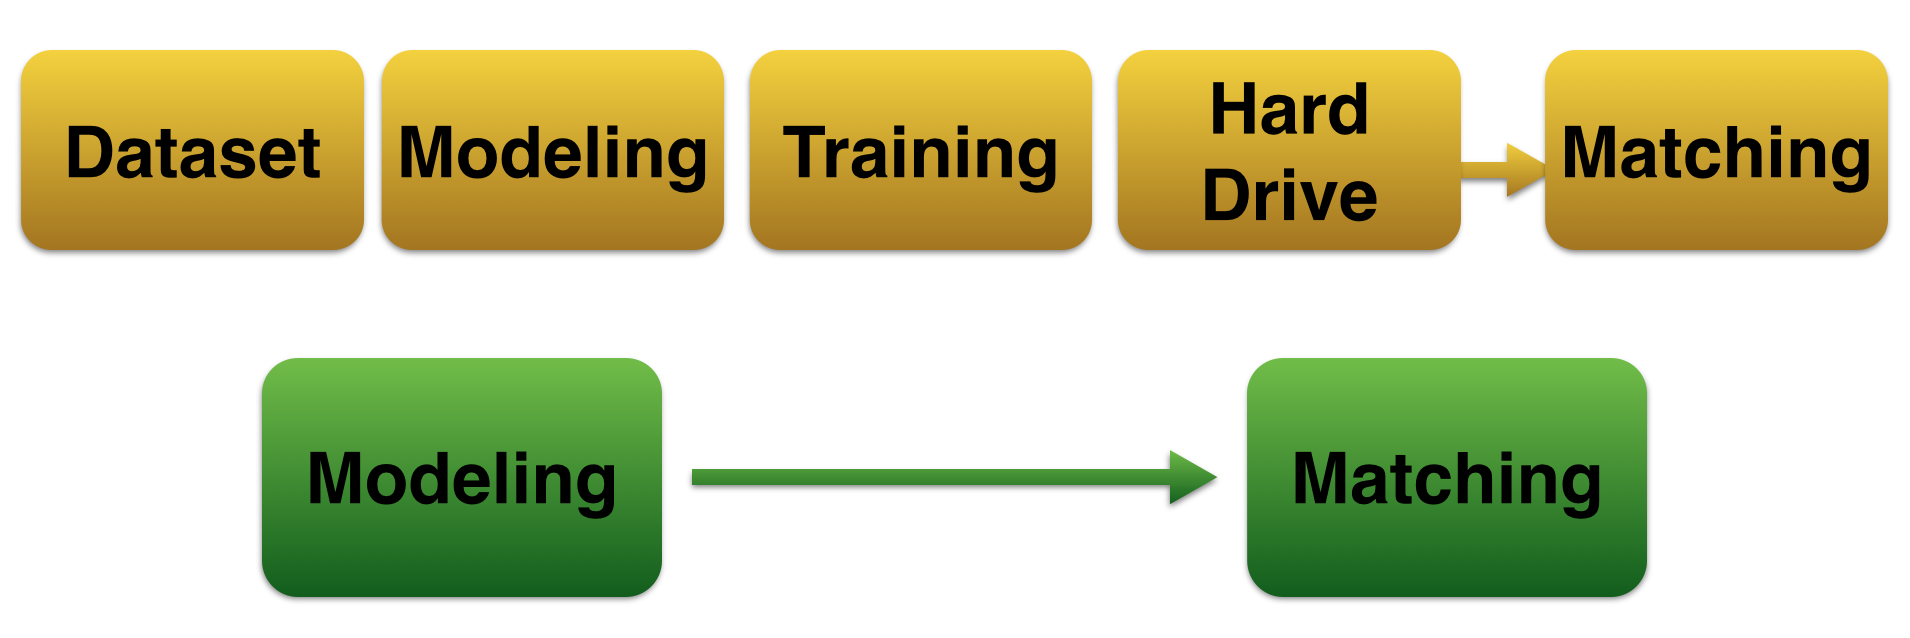
\includegraphics[width=0.9\linewidth]{schematics} 
  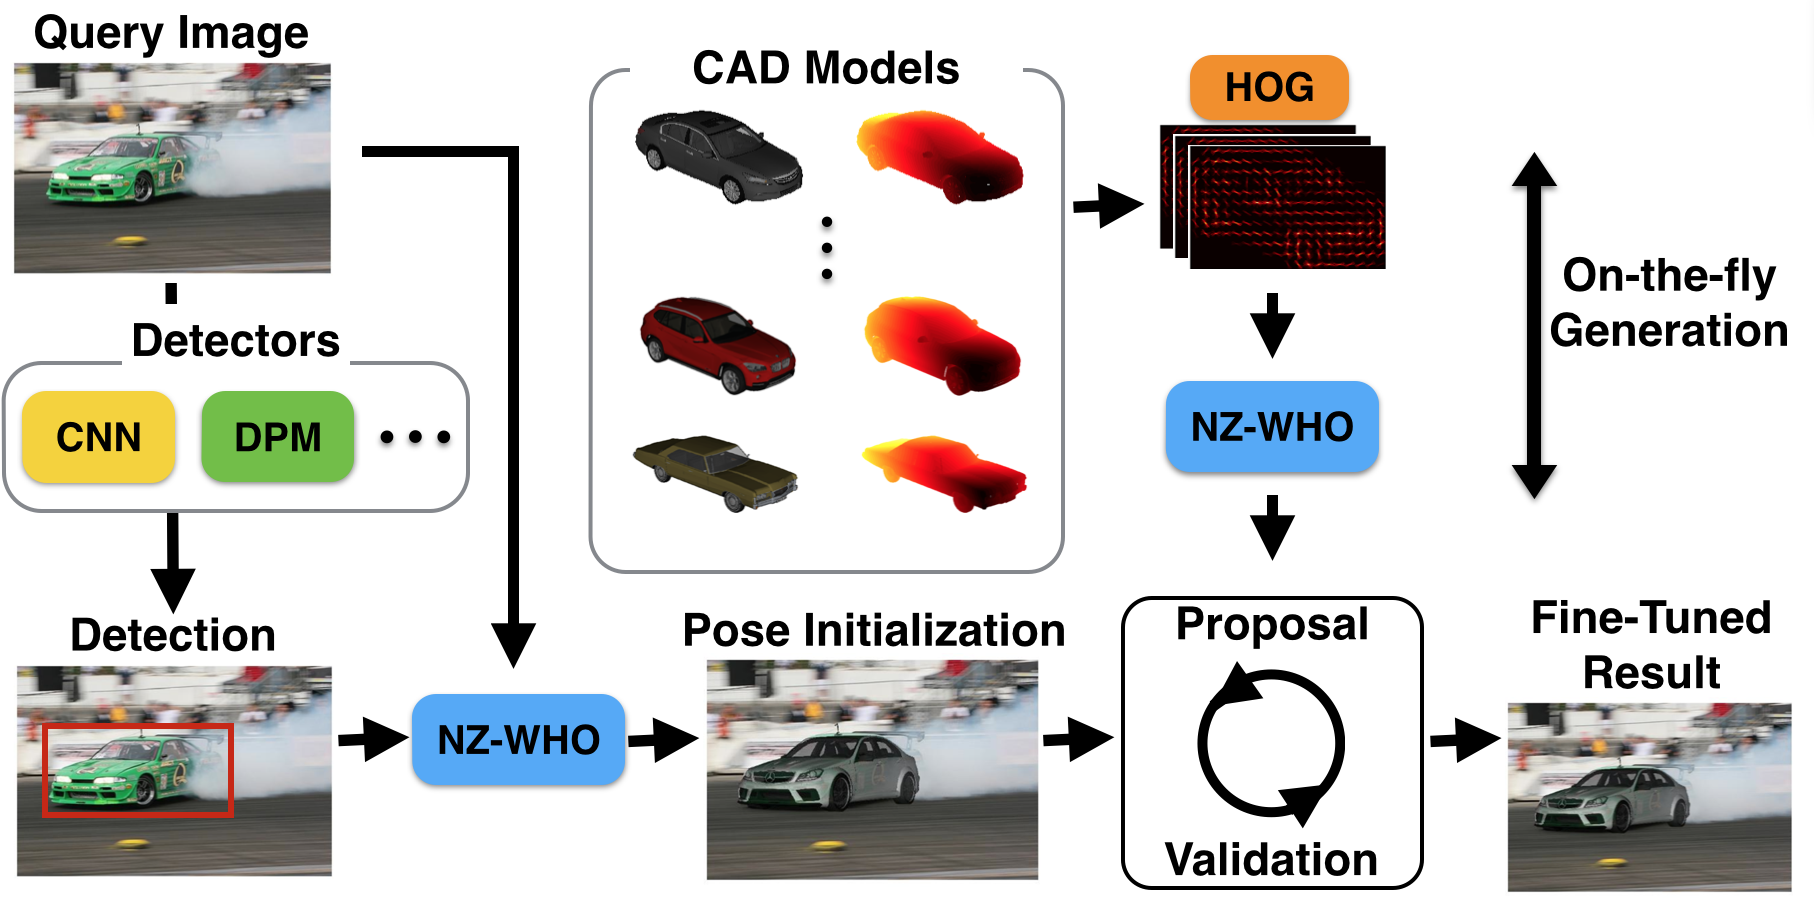
\includegraphics[width=0.99\linewidth]{front} % \\[-5pt]
  % (a)\\[0pt]
  % \setlength\tabcolsep{0pt}
  % \begin{tabular}{cc}
  %     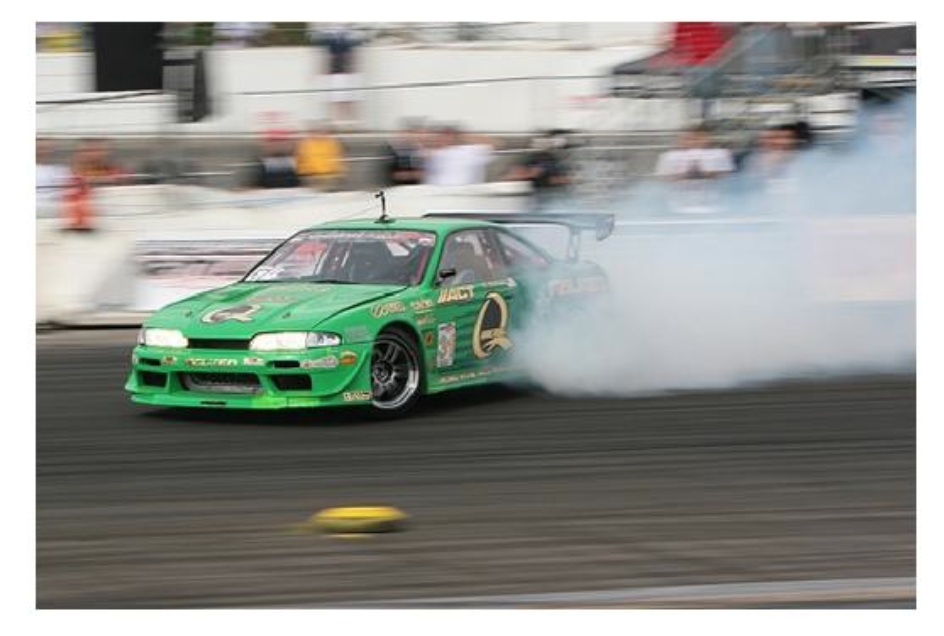
\includegraphics[width=0.45\linewidth]{car/orig2} & 
  %     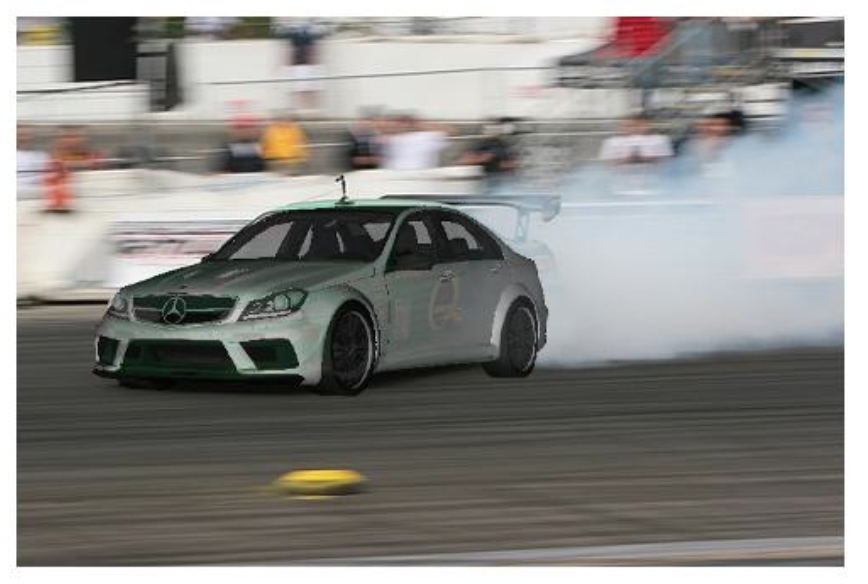
\includegraphics[width=0.45\linewidth]{car/overlay2}
  %  %   \begin{tabular}{cc}
  %  %       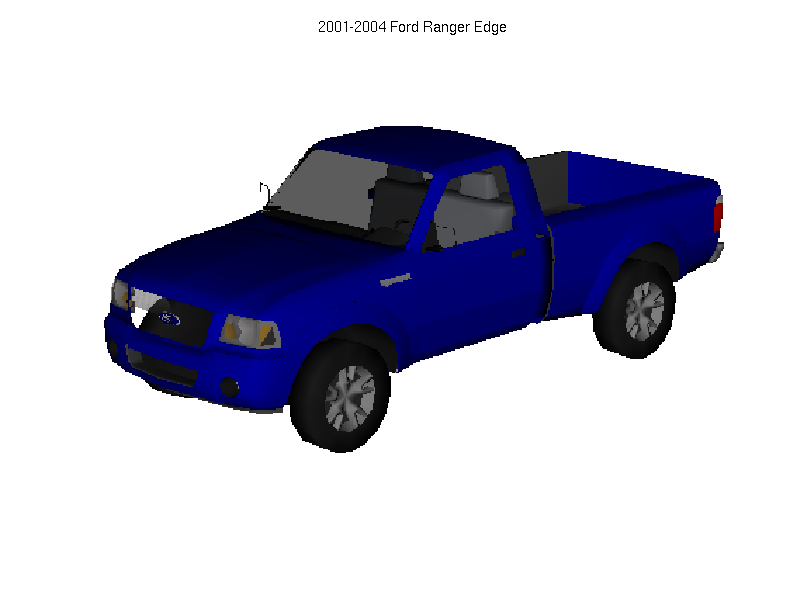
\includegraphics[width=0.16\linewidth]{cad_car/2001-2004 Ford Ranger Edge} & 
  %  %       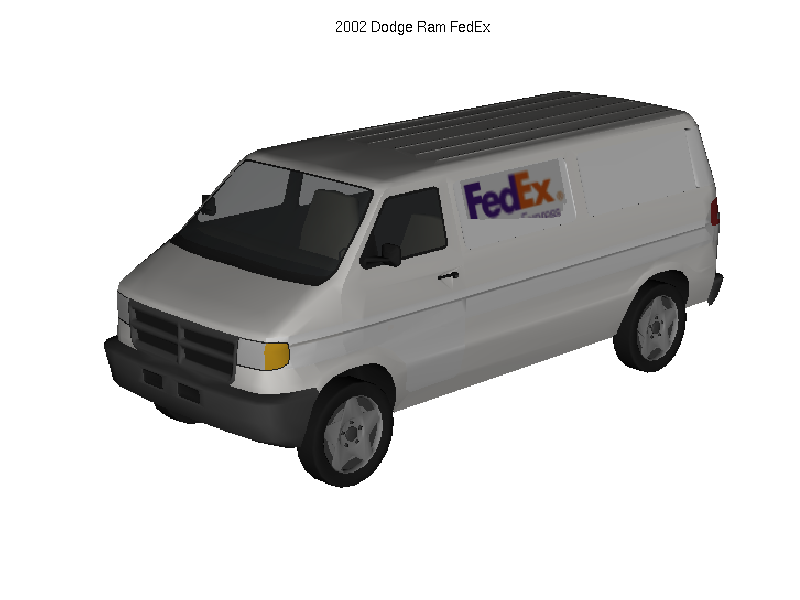
\includegraphics[width=0.16\linewidth]{cad_car/2002 Dodge Ram FedEx} \\ 
  %  %       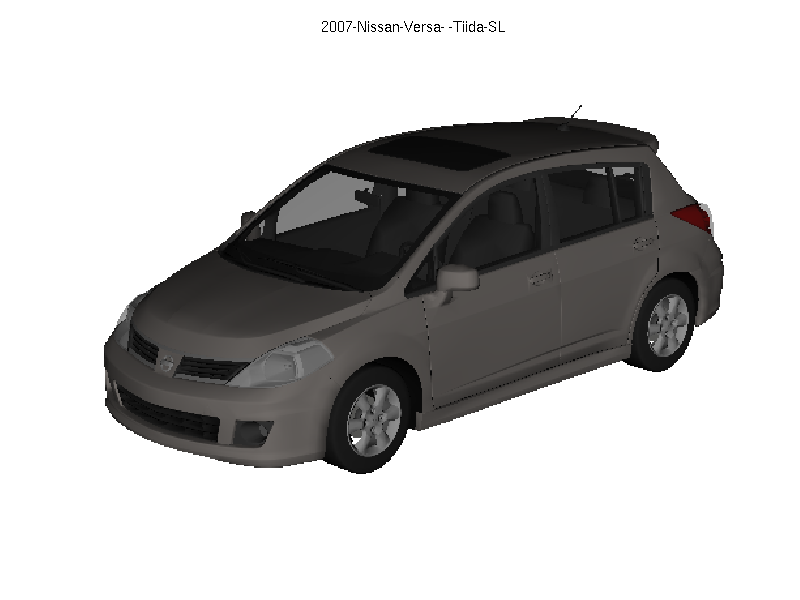
\includegraphics[width=0.16\linewidth]{cad_car/2007-Nissan-Versa-_-Tiida-SL} & 
  %  %       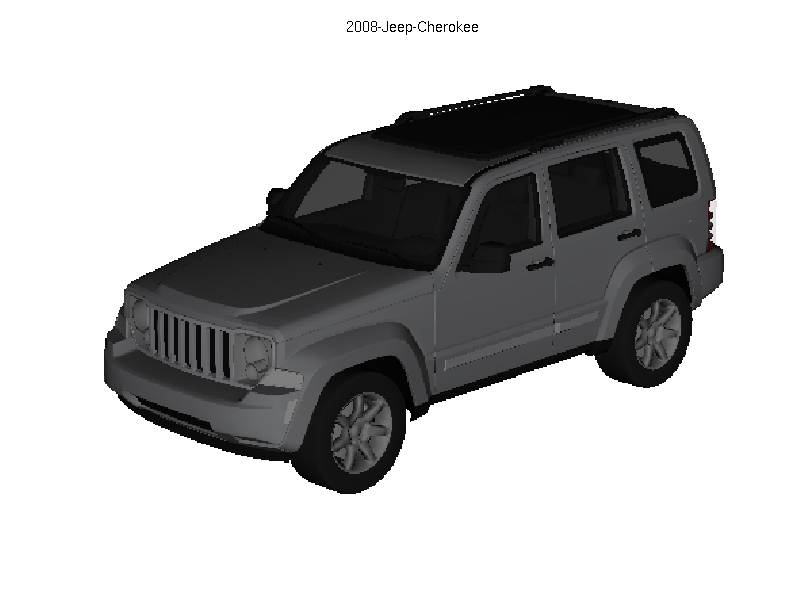
\includegraphics[width=0.16\linewidth]{cad_car/2008-Jeep-Cherokee} \\ 
  %  %       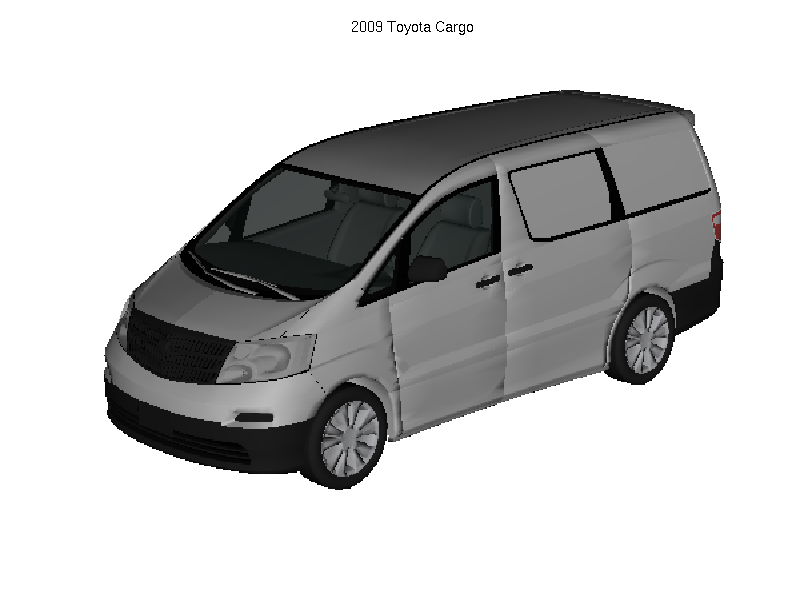
\includegraphics[width=0.16\linewidth]{cad_car/2009 Toyota Cargo} & 
  %  %       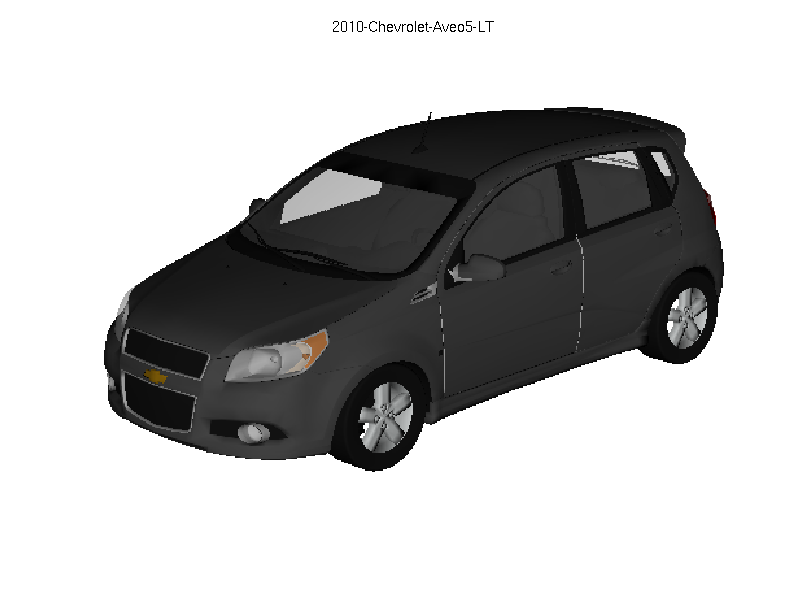
\includegraphics[width=0.16\linewidth]{cad_car/2010-Chevrolet-Aveo5-LT} \\ 
  %  %       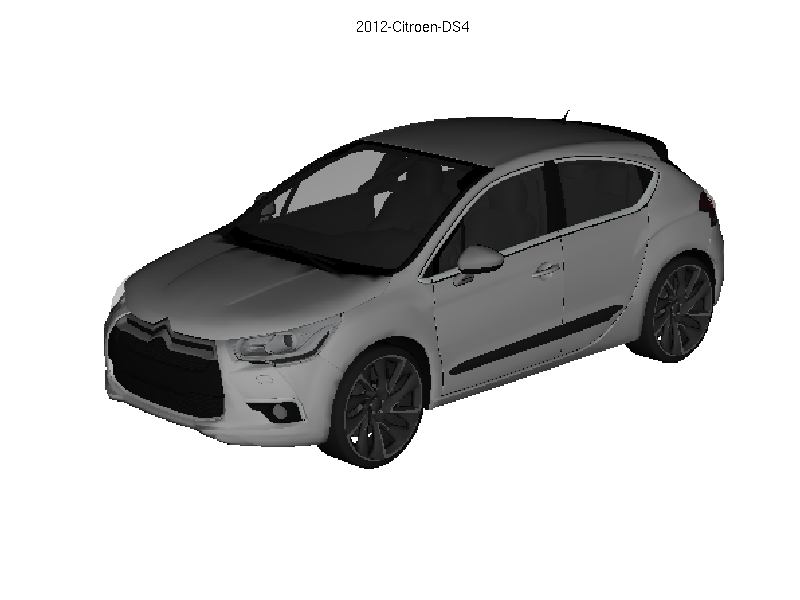
\includegraphics[width=0.16\linewidth]{cad_car/2012-Citroen-DS4}  
  %  %   \end{tabular}
  % \end{tabular}\\
  % (b)
  \caption{Using a bank of CAD models, we generate NZ-WHO templates which can be used to either detect objects directly or initialize pose of an object in the bounding box from other detectors. Once initialization is given, we use NZ-WHO to propose and validate plausible pose on-the-fly and further tune the translation, 3D viewpoint and focal length continuously.}
  % \vspace{-1em}
  \label{fig:front}
\end{figure}
 
% Object detection task has long been about predicting rectangular bounding boxes around the object. In this workthere has been significant many powerful object detectors such as Convolutional Neural Network or Part-Based Models \cite{Girshick14, Felzenszwalb10, Pepik12} 

Current approaches to object class detection have reached a remarkable
level of performance in 2D bounding box
localization~\cite{pascal12,Felzenszwalb10,Girshick14}, due to their
ability to generalize across differences in object appearance,
lighting, and viewpoint. While this generalization
ability of these methods is benefitial for robustness, it also limits
the level of detail that these detectors can deliver as an output.

As a consequence, there has been increased interest in multi-view object
recognition, where viewpoint estimates are provided by
detectors in addition to 2D bounding boxes. Several attempts have been
made to estimate viewpoint along with object class detections,
implemented as extensions to existing detectors, such as the implicit
shape models~\cite{}, the constellation model~\cite{}, or the
deformable part model~\cite{Xiang12,Pepik12,Fidler12,Hejrati14}.

Recently, an even higher level of geometric detail was reached in the
form of aligning
3D CAD model instances to real world test images~\cite{Aubry14,
  Lim14,Kholgade14, Chen13, Kostas14}. Interestingly, the problem of matching 3D models to 2D
images has been targeted since the early days of computer
vision~\cite{Lowe87}, but had largely been neglected in recent years
in favor of 2D detectors based on robust local features and
statistical learning techniques. Now, this problem is being revisited
mostly due to two reasons: {\em (i)} the availability of 3D CAD models
for many object classes and {\em (ii)} the availability of robust
image matching techniques.
%
% performance object detectors usually generalizes very well. It
% can handle various intraclass variability, viewpoint change and
% occlusion. However due to this high generalization, sometimes it is
% very difficult to get accurate pose, category or 2D-3D matching. Our
% method, specialized in giving such accurate information, can be
% applied on any generic object detectors to give high quality metadata.
% %
% Matching 3D CAD model to an image has been a classical problem that
% dates back to eighties . Lowe \etal , the vision
% community instead focused on the object detection tasks that estimates
% a rectangular bounding box around an object\cite{Felzenszwalb10,
%   Girshick14}. 
%
%In addition, there has been a growing emand for accurate 2D-3D
%matching \cite{Kholgade14, Chen13, Kostas14} for image manipulation,
%editing, and data augmentation in the computer graphics community.
%
% Recently, with the powerful computing capabilities and a large
% collection of CAD models, the 2D-3D matching (registration) problem
% gets more and more approachable but due to inherent difficulty and
% limited performance of existing methods, many applications still
% require supervision to achieve 2D-3D matching.
% In medical community, registering 3D scan data to 2D image enabled various minimally invasive surgeries \cite{Markelj12}.
%
% For category-level matching, \cite{Xiang12, Hejrati14, Pepik12} used
% 3D parts or aspect to represent underlying category-level 3D geometry
% of the object. With the advent of large public CAD datasets
% \cite{Trimble, Yobi}, the instance-level object detection and 2D-3D
% registration became possible. \cite{Aubry14, Lim14} used large
% collection of CAD models to faithfully align 3D CAD model to an image
% by rendering CAD models and creating 2D templates for various
% viewpoints.

For (i), recent approaches to 2D-3D matching~\cite{Aubry14, Lim14}
typically rely on a
collection of 3D exemplar models, which they render from a
large number of viewpoints. The resulting artifial images are then
used to train exemplar models that can be matched to a real-world
image at test time.
%
For (ii), it has been realized that template-based exemplar detectors
based on HOG~\cite{Dalal05} features can be trained analytically, by
replacing the standard SVM with an LDA classifier
(E-LDA)~\cite{Hariharan12}. As a result, it is feasible to train
hundreds of thousands of mid-level patch detectors for
recognition~\cite{Aubry14}.
%
Unfortunately, the performance of E-LDA relies crucially on an
additional calibration step that equalizes the detection scores of
independently trained exemplar models. Since this step involves costly
mining of hard negative examples~\cite{Dalal05,Felzenszwalb10} on a
validation set, it constitutes the major computational bottleneck of
E-LDA, limiting its scalability.

In this paper, we propose a novel method for 2D-3D alignment of
exemplar CAD models to real-world images that circumvents the need for
calibration, and greatly enhances the scalability of E-LDA. As a
result, we can render novel views and train corresponding exemplar
models {\em on the fly}, without the need for offline processing. As a
by-product, we can formulate the alignment problem as a parameter
search in a continuos pose space, consisting of azimuth, elevation,
and ~\scream{}, resulting in truely continuous pose estimates, which
we implement using MCMC sampling.
%  require a large number of rendering and 2D
% templates for each of the CAD model with specific viewpoint. Since
% there are so many templates that it becomes almost impossible to get
% all the true positive image from training data. Instead \cite{Aubry14,
%   Lim14} used whitening as a preprocessing stage \cite{Hariharan12} to
% make templates more discriminative. Then calibration is done on a
% small training dataset.
%
% Although whitening to create template is faster than some of
% instance-level matching algorithms such as training Exemplar-SVM
% \cite{Malisiewicz11} or complicated models such as LEVAN
% \cite{Divvala14}, whitening and calibration large number of templates
% takes very long time. Also, once the fixed discrete viewpoint
% templates have been made and calibrated, it is difficult to fine-tune
% the prediction made using the large collection of templates.

Our paper makes the following specific contributions.

First, we present a novel method for training exemplar models from
rendered 3D CAD data {\em on the fly}, enabled by a novel variant of
E-LDA, and making efficient use of the specific characteristics of
rendered images. To our knowledge, our method constitutes the first
attempt to simultanously render and train exemplar detectors on the
fly.
% In our paper, we present Non-Zero Whiten Histograms of Orientations
% (NZ-WHO) to dramatically speed up the template generation and get rid
% of time consuming calibration and yet achieves performance on par with
% calibrated templates. First, we will present NZ-WHO is more
% discriminative than WHO and introduce Conjugate Gradient method to
% speed up the whitening and create a high resolution template in just
% 80 milliseconds. Also, using this fast NZ-WHO template generation, we
% present \textbf{on-the-fly} template generation to fine tune an
% initial pose estimation to continuously refine translation, viewpoints
% (yaw, roll, pitch) and focal length.

Second, we show to enrich the output of an existing object class
detector, such as the DPM~\cite{Felzenszwalb10} or the
R-CNN~\cite{Girshick14} with additional 3D information, applying our
method to candidate detections provided by the respective detector. As
a result, we can refine the original detections with additional
estimates of 3D continuos pose and a 3D CAD model exemplar.

And third, we give an in-depth experimental study that demonstrates
the effectiveness of our approach on a standard benchmark for
object detection and viewpoint estimation~\cite{Xiang14}. 



outperforming previous results on this dataset by considerable
margins.



%% Our contribution
With this growing usage of WHO template and Computer Graphics
rendering, we decided to analyze WHO feature
[Find More Usage of WHO and CG rendering \cite{Pepik12}]




Our pipeline is simple, fast only requires CAD models and no
validation images for calibration. This can be used for post
processing stage of generic object detection. Our pipeline requires
only several minutes to make templates for rough viewpoints and 


We propose a simple method to register the most similar CAD model to
an image and fine-tune viewpoint continuously without discriminative
part search, training nor calibration. Our method is simple, fast and
light-weight in terms of memory so that it can be easily applied on
top of generic object detectors as a final stage of detection or can
be used as a standalone detector. 



% Although our method is geared toward instance-level 2D-3D matching, we evaluated the performance of the templates on PASCAL 2007 and PASCAL 2012 and PASCAL 3D dataset to measure the performance. 

Our tuning stage not only refine position, scale and viewpoint, but
also focal length as well to literally "fine-tune" the initial
proposal. Though our 2D-3D matching method can be used as a
rudimentary object detector, our simple tuning stage can be applied to
any generic object detector to achieve state-of-the-art viewpoint
estimation method.


Finally, we show several applications using our method. Since we have
metadata such as CAD model and geometry, we reconstruct the object
using 2D-3D matching. Also, since we do not need training image, we
show that our 2D-3D matching performs better than standard detectors
in categories where training data lacks. We then use our method for
image query to pull out closest CAD model in a bank of CAD models.


Finally, unlike several CAD model alignment methods that uses  WHO
\cite{Aubry13, Aubry14, Lim14}, we propose a novel pipeline that does
not require calibration which is infeasible in continuous viewpoint
estimation. We propose a simple add-on stage that can enrich object
detections with high-quality 2D-3D alignment. The pipeline is simple
and light weight so this can be easily adapted to be used for any
generic object detectors. Also to facilitate the future work, all our
alignment result on PASCAL12 and code are publicly available online.




% Recently, matching a 3D CAD model to an image, 2D-3D matching (registration), is gaining great momentum in various fields of study. 2D-3D matching using Structure from Motion \cite{Sattler11} uses existing 3D model to match the model to a query image. Also image manipulation using 3D CAD models has proven its potential. Kholgade \etal \cite{Kholgade14} and Chen \etal \cite{Chen13} require human input to match 3D models to an image to created realistic morphing or manipulation of the registered object. However, all these application requies human input. In this paper, we propose a novel on-the-fly template generation algorithm that can generate template quickly and validate 2D-3D pose and focal length continuously.

% Our code has been made publicly online \cite{Choy14} so that our algorithm can be used as a pipeline for 2D-3D registration after general purpose object detectors.


\subsection{Approach Overview}
Our method is in line with \cite{Aubry14, Lim14} in the sense that we
use only renderings not real images. However, rather than using fixed
sized mid-level patches, we use whole object and make root
templates. By using root templates, there is no need to learn a
discriminative patch dictionary or to calibrate the patches and an
additional inference stage is not required. However, whitening the
whole template is prohibitive for several reasons. All templates have
different aspect ratios making it difficult to generate the covariance
matrix $\Sigma$. Since the root templates are larger than mid-level
patches, a very large auto-covariance $\Gamma$ is required. Lastly,
time complexity of decorrelating a template with $n$ cells increases
as $O(n^3)$, resulting in slow template generation and large residuals
due to numerical errors accumulated while decomposing the covariance
matrix $\Sigma$. 

To overcome these difficulties, we propose the Non-Zero Whitened
Histograms of Orientations with iterative Conjugate Gradient to
generate templates in real time and enrich rectangular boxes with high
quality 2D-3D matching. The 2D-3D matching provides a CAD model,
sub-category, rendering, depth, viewpoint and focal length.

Our method can work as a standalone 2D-3D matching algorithm, or even
as a standalone ensemble of exemplar-based object detectors (Figure
\ref{fig:front}) but the real power comes from combining generic
object detectors and complement rectangular bounding boxes. Our method
is simple in design; is several orders of magnitude faster than
traditional method; requires only CAD models; doesn't need images nor
calibration, yet is powerful in giving high-quality metadata. These
properties make our method ideal for complementing object detections. 

To complement detection bounding boxes, we first search possible 2D-3D
matching by running cached discrete viewpoint templates. Then, for the
most probable match, we refine the initial matching using Metropolis
Hastings. Since it requires iterations of proposal and validation, we
present real time analysis of NZ-WHO template generation to show that
this can be done on-the-fly. The fine tuning stage process jointly
optimizes translation, yaw, roll, pitch, scale, and focal length
continuously and also searches for different CAD models.






\section{Related Works}
\subsection{Whitened Histograms of Orientations (WHO)}
% History of Whitening and how whitening works
Recently, Hariharan \etal. introduced Whitened Histograms of Orientations (WHO) \cite{Hariharan12}, which used statistics from natural images to whiten HOG templates, making them more discriminative. Whitening is a common signal processing operation for decorrelating a set of random variables \cite{Martinsson05, Belouchrani00}. More formally, suppose that we have a $k$-dimensional random variable $X \in \mathcal{R}^k$ with $Cov(X)=\Sigma$. By whitening the signal, i.e., $\tilde{X}=\Sigma^{-\frac{1}{2}}(X - E[X])$, we remove 2nd order correlation between all features. So, all elements in the random variable $\tilde{X} = \left[\tilde{X}_1, \tilde{X}_2, \dots, \tilde{X}_k\right]$, become more independent. In the context of HOG features, a whitened HOG template will produce Gaussian noise when convolved with a random natural image, but a delta-like response on an image matching the template. WHO templates are more discriminative than standard HOG templates because they only capture the gradients that differentiate the object from random images. \scream{chris added the following} Hariharan \etal. also interpreted the whitening as Linear Discriminant Analysis (LDA) where all classes have different means but have the same covariance. The whitening and LDA have the same formulation when we make a decision boundary $w = \Sigma^{-1}(\mu_+ - \mu_0)$ where $\mu_+$ is the features from a class (LDA) or a signal to whiten (whitening), $\mu_0$ is the negative class center (LDA) or a signal statistics (whitening) and $\Sigma$ is the covariance matrix of classes (LDA) or correlation within signal (whitening).

\textcolor{red}{Should we mention how our method improves on this (ie by using CG)?}

% Using HOG
% In this paper, we also used Histograms of Orientations feature \cite{Dalal05} but in general, we could use any dense features. 

\subsection{Object Detection and Viewpoint Estimation}

Modern object detectors generalize very well, handling intraclass variability, occlusion, truncation and viewpoint changes \cite{Felzenszwalb10, Girshick14}. However, this generalization comes at the cost of fine-grained information, including accurate 3D pose and object sub-category recognition. Such methods typically produce bounding box detection hypotheses, with little further information.

Many methods have attempted to move object detection towards richer outputs, especially by jointly performing detection and pose estimation \cite{Pepik12, Xiang12, Fidler12, Xiang14, Hejrati14, Aubry14, Lim14}. To achieve this, \cite{Xiang12, Hejrati14, Fidler12} use 3D representations that deform as viewpoint changes and \cite{Pepik12} uses geometric constraints to regularize 2D appearance models.

The methods above perform discrete pose estimation, quantizing the viewing sphere into a number of poses and selecting the best one during inference. Fine-grained pose estimators, in contrast, can infer continuous (or arbitrarily fine-grained) poses. One such method from \cite{Zia13} aligns a 3D deformable part-based wireframe model with input images to accurately predict object poses.

More recently, \cite{Aubry14, Lim14} made progress in joint instance-level object detection and pose estimation. To estimate pose they use synthetic renderings of CAD models to learn discriminative mid-level patches. \cite{Aubry14} calibrates these patches on a small set of real images, while \cite{Lim14} present a method for learning the relative discriminativeness of the patches.

\textcolor{red}{Again, should we highlight the differences between these methods and ours?}

% specialized in giving such accurate information, can be applied on any generic object detectors to give high quality metadata.
% Many 
% Since the WHO does not require extensive training such as \cite{Felzenszwalb10, Malisiewicz11, Girshick14}, WHO is gaining momentum in 2D-3D matching. \cite{Aubry13, Aubry14, Lim14} combined WHO with synthetic rendering to jointly detect and estimate pose by making mid-level patches using WHO. Using this
% WSuch approach has an advantage over generic detections. First, it is easy to trace the detection to specific template. The template also has The rendering has corresponding CAD model and viewpoint thus enabling joint detection and viewpoint estimation. 
% To deal with textureless background \cite{Aubry13} whitens HOG feature and then zero out the WHO feature where there is no texture. But centering a HOG feature where there is no edge creates strong negative edges. We found out that centering only non-zero cells help detection but whitening all cell makes features to leak out to texture-less regions.
% With increasing popularity of rendering image, whitening, traditional signal processing technique, as a preprocessing stage has been widely used also in computer vision community.
% Many object detectors \cite{Felzenszwalb10, Malisiewicz11}
% \subsection{Mid-level Patches for 2D-3D matching}
%  FPM introduction : per instance matching  
%  Seeing 3D chair : mid-level patches
  
%\begin{comment}
%  \subsection{Contributions}
 % \begin{enumerate} \itemsep1pt \parskip0pt \parsep0pt
  %  \item Introduces Non-Zero Whitened Histograms of Orientations (NZ-WHO) for real-time template generation
   % \item Continuous viewpoint and focal length tuning using on-the-fly template generation
%    \item Jointly optimizes translation, 3D viewpoint, CAD models and focal length
%     \begin{comment}
%       \item HOG Whitening procedure that do not require calibration stage
%     \end{comment}
%  \end{enumerate}
% \end{comment}
% All the code and CAD models is publicly available online \cite{Choy14} (currently not disclosed for anonymous review, visualizations are available in the supplementary material).

\section{2D-3D Matching using Non-Zero Whitened Histograms of Orientations(NZ-WHO)}
\label{sec:nz-who}

We propose Non-Zero Whitened Histograms of Orientations (NZ-WHO), that are both more discriminative than WHO, and can be generated in 70ms (compared to several seconds for WHO). This speed up means we can generate templates on the fly, allowing our approach to evaluate arbitrary viewpoint hypotheses. 
\scream{chris:We propose Non-Zero Whitened Histograms of Orientations (NZ-WHO), an improvement over WHO which is both more discriminative than WHO and can be computed many orders of magnitude faster than WHO (70ms as opposed to to several seconds for WHO). This speedup allows us to generate NZ-WHO templates on the fly, allowing us to quickly evaluate arbitrary viewpoint hypotheses.}

The computational efficiency of our approach comes from using the iterative conjugate gradient method to whiten the HOG template. Whitening a feature vector $x$ requires a system of linear equations $\Sigma w = (x - \mu)$ to be solved, usually by decomposing the covariance matrix $\Sigma$ (with LU or Cholesky decomposition). Since the covariance matrices of HOG templates have nice spectral properties (see Section \ref{sec:fast_whitening}), the conjugate gradient method will converge to the solution several orders of magnitude faster than decomposition methods.

Our second innovation is 'Non-Zero' whitening. When synthesizing detection templates from rendered images, a common problem is how to handle the background. If we render the model over a natural image background, gradients in the background will be incorporated into the discriminative template. Alternatively, we could leave the background textureless \scream{did Hariharan do this?} (see Fig.~\ref{fig:rendering}), but whitening the resulting HOG template produces in undesirable background artifacts. These are created when centering the template (by subtracting the mean $\mu$), where strong negative weights are introduced in the textureless region (as seen in Fig.~\ref{fig:whocomparison}). This could result in positive matches being suppressed due to spurious background gradients.

To remove such artifacts, we construct $x$ using only cells with non-zero gradients. After whitening we restore the full template, with the zero-gradient cells left unchanged. This approach has the added benefit of reducing the size of the linear system we need to solve, further speeding up our method.

Table \ref{tab:who_initializations} provides a detailed comparison of WHO and NZ-WHO templates, illustrating that our method is faster and more discriminative than Whitened Histograms of Orientations. \scream{Does the table show this?}

% We compare the performance of WHO and NZ-WHO on 3D Object dataset \cite{Savarese07} and report performance on Table \ref{tab:who_initializations}. 

% To deal with the problems, we propose Non-Zero Whitened Histograms of Orientations.

% To accommodate the growing usage of rendering image for 2D-3D matching using WHO\cite{Aubry13, Aubry14, Lim14}, we analyzed various methods to whiten synthetic rendering image and propose Non-Zero Whitened Histograms of Orientations (NZ-WHO) which is a direct extension of \cite{Hariharan12} designed for rendering images with textureless background. % Since a NZ-WHO template has zero-mean and all elements in the template follow same distribution, no explicit calibration is required if all the templates have approximately the same number of cells. 

% Since Combining NZ-WHO with Conjugate Gradient, 

% \subsection{Non-Zero Whitened Histograms of Orientations (NZ-WHO)}
% why non zero whitening and why it makes more sense than seeing 3D, IKEA
% Overview of the subsections
%   Generating covariance quickly
%   Fast inversion
%   Regularization

\begin{figure}[t]
  \begin{center}
%   \fbox{\rule{0pt}{2in} \rule{0.9\linewidth}{0pt}}
    % include whitening all centered cells
    % 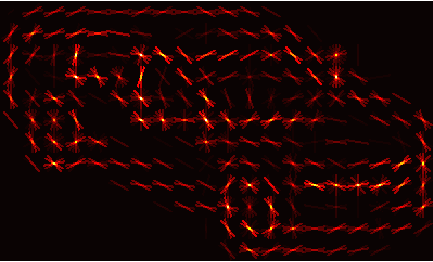
\includegraphics[width=0.32\linewidth]{whiten_all_crop}
    \setlength\tabcolsep{3pt}
    \begin{tabular}{ccc}
      HOG & WHO & NZ-WHO \\
%     \begin{turn}{90}$w_+$\end{turn} &
    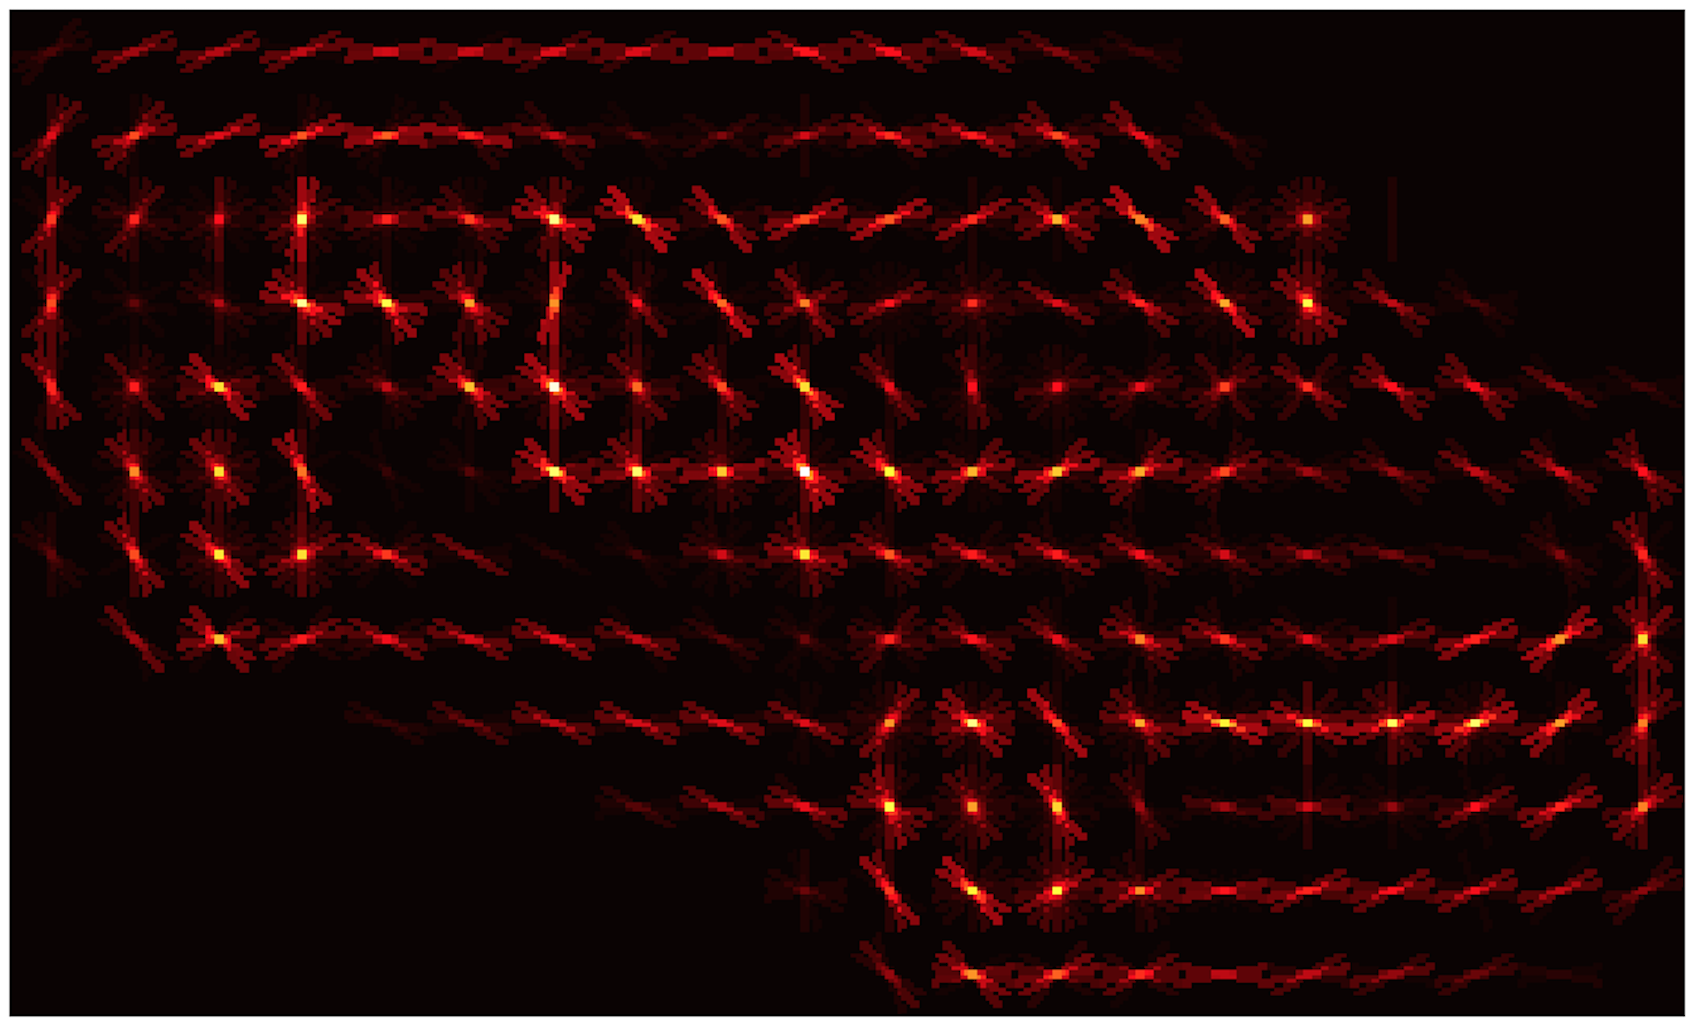
\includegraphics[width=0.28\linewidth]{hog_crop} &
    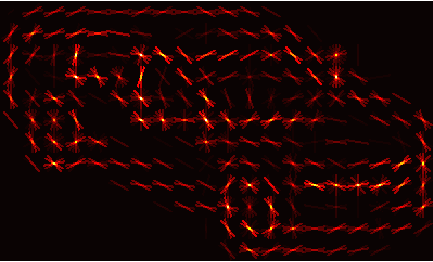
\includegraphics[width=0.28\linewidth]{whiten_all_crop} &
    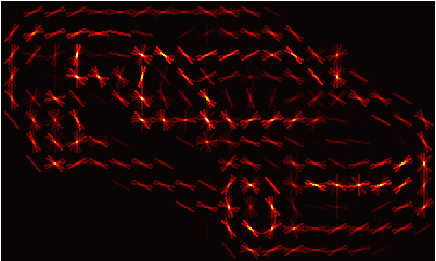
\includegraphics[width=0.28\linewidth]{whiten_non_zero_crop} \\
    % include whitening all centered cells
     % 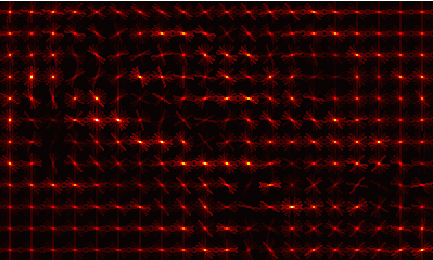
\includegraphics[width=0.282\linewidth]{whiten_all_neg_crop} 
%     \begin{turn}{90}$-w_-$\end{turn} &
     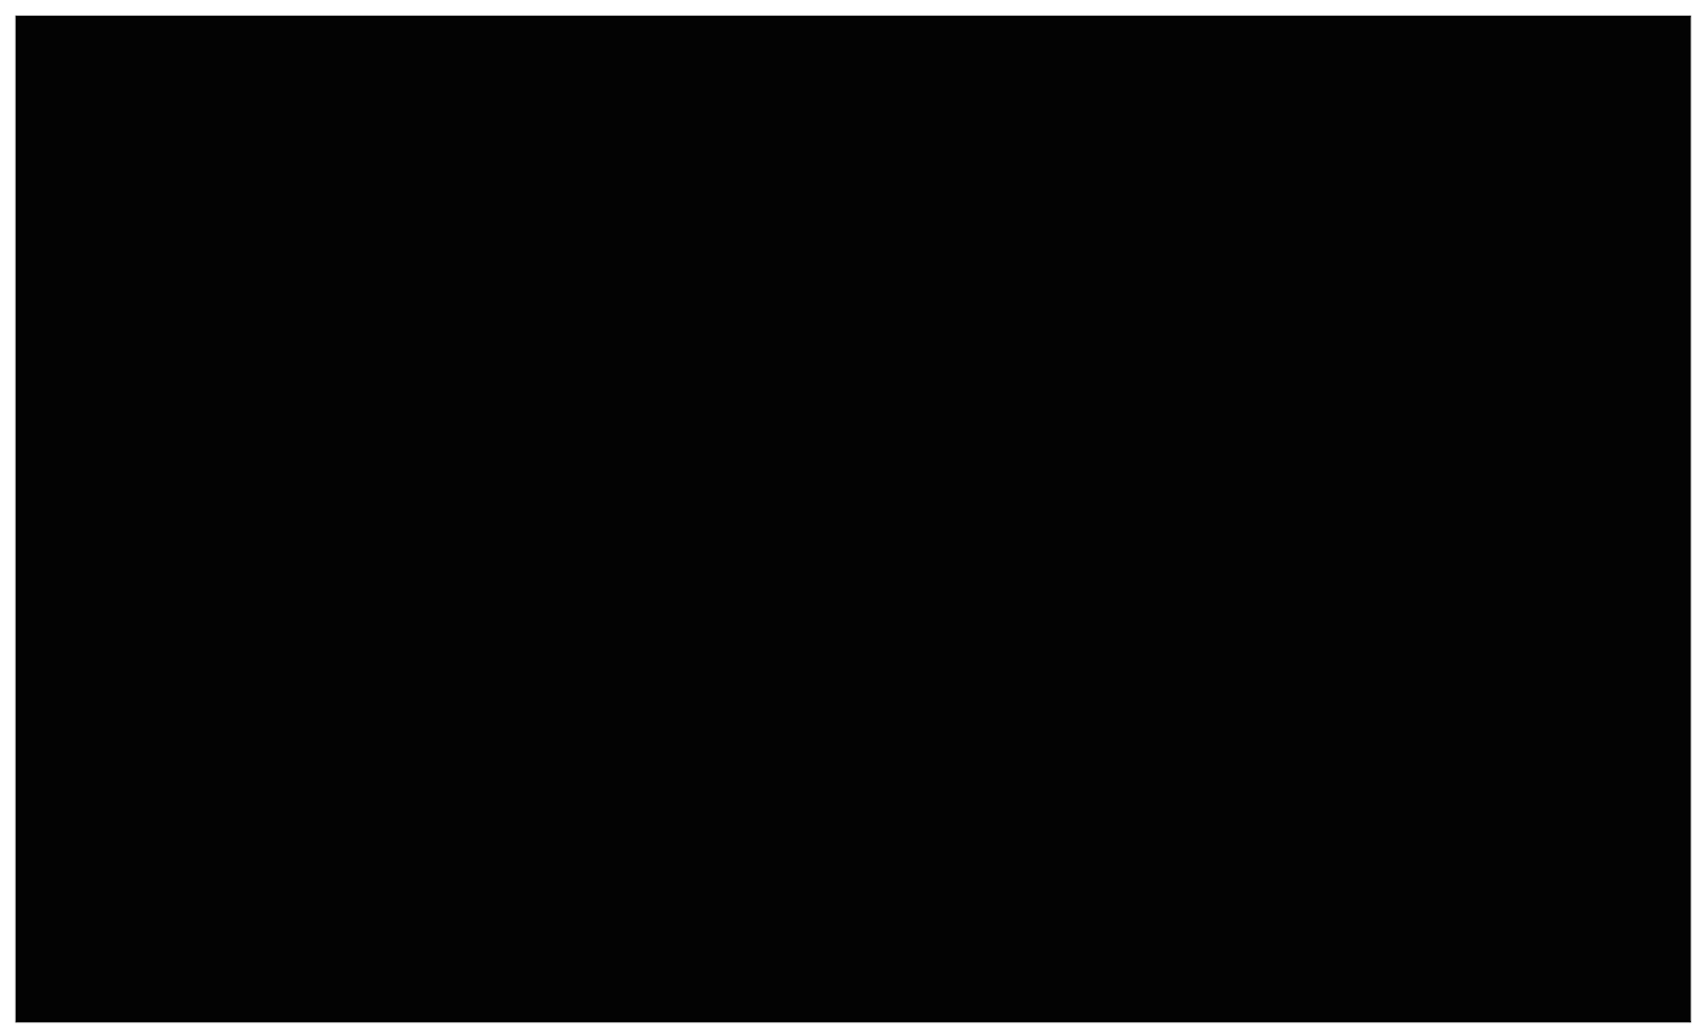
\includegraphics[width=0.28\linewidth]{hog_neg_crop} &
     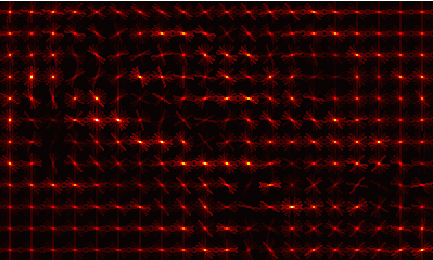
\includegraphics[width=0.28\linewidth]{whiten_all_neg_crop}  &
     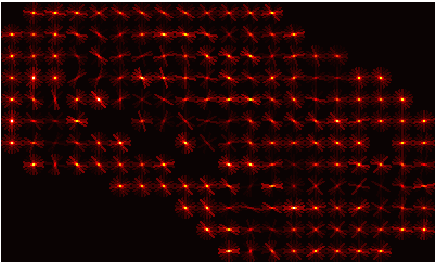
\includegraphics[width=0.28\linewidth]{whiten_non_zero_neg} \\
    % include whitening all centered cells
 %    \begin{turn}{90}ihog\cite{vondrick2013}\end{turn} &
    % \cite{vondrick2013}& 
     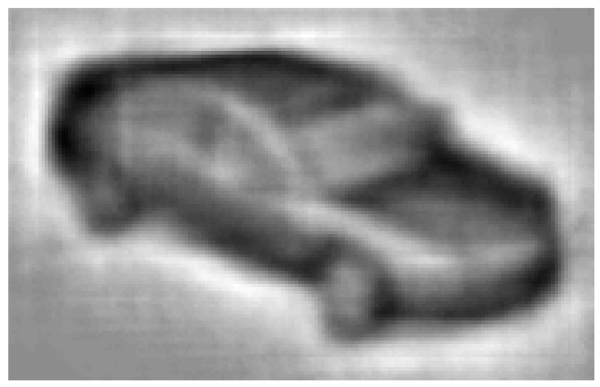
\includegraphics[width=0.28\linewidth]{ihog_hog200_crop.png} &
     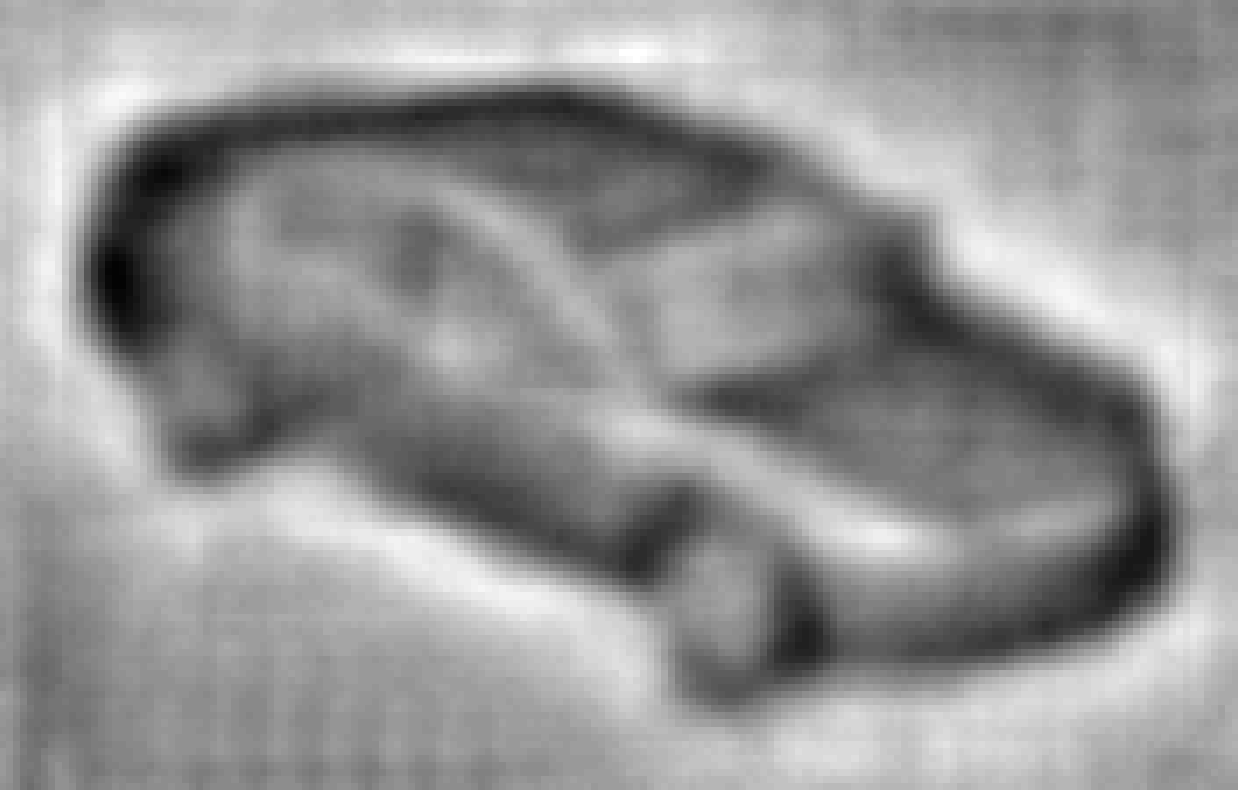
\includegraphics[width=0.28\linewidth]{ihog_whiten_all200_crop.png} &
     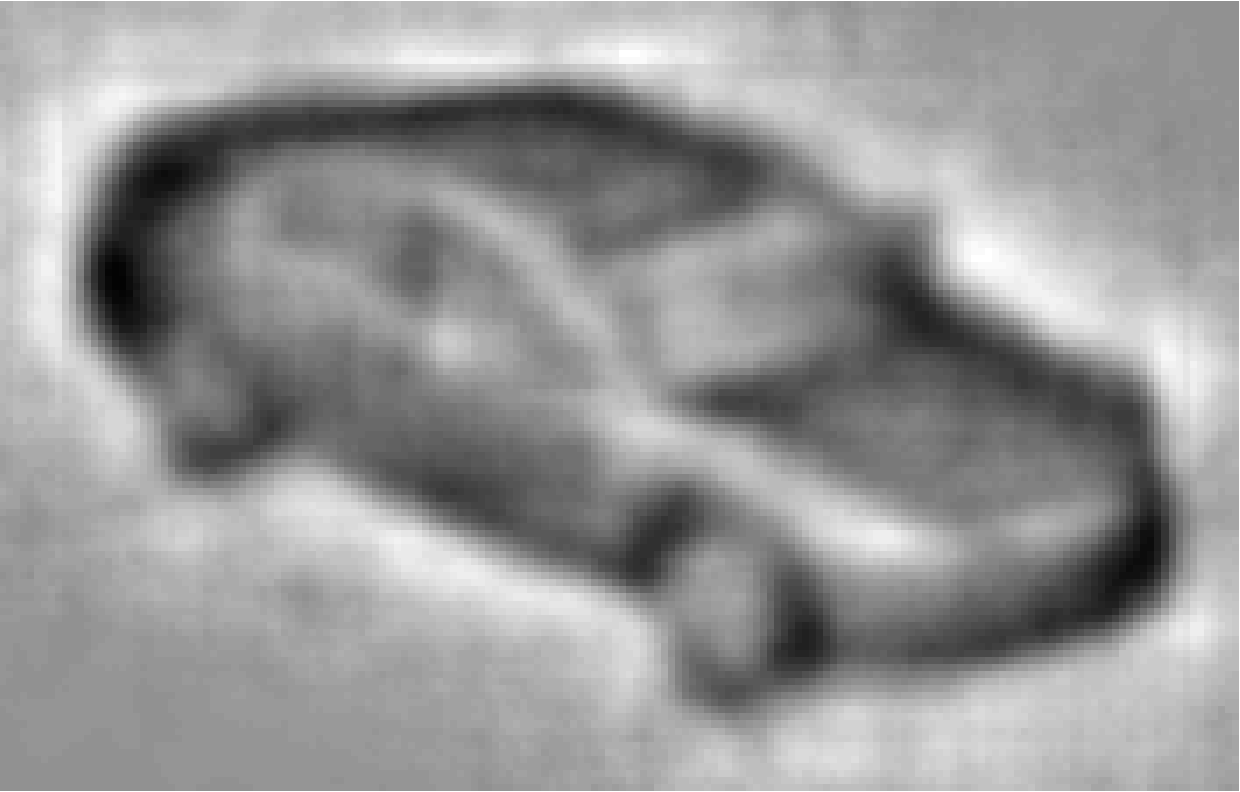
\includegraphics[width=0.28\linewidth]{ihog_whiten_non_zero200_crop.png} \\
 \end{tabular}
  \end{center}
  \caption{Comparison of HOG, WHO and NZ-WHO. Visualization of positive weights (first row),  visualization of negative weights (second row), HOGgles \cite{vondrick2013} (third row). Note that for WHO, whitening all cell result in strong negative edges on the empty region}
  \label{fig:whocomparison}
\end{figure}

% Overview of the subsections
% In this section, we will give a brief overview of whole whitening stages. In the first section \ref{feature_statistics}, we will discuss about first and second order statistics of HOG feature. Then, we will discuss about using autocovariance $\Gamma$ to create covariance matrix $\Sigma$ for non-zero cells and SIMD implementation to speed up the generation. Then, we will explain fast and accurate way to solve $w = \Sigma^{-1}x$ using Conjugate Gradient method. % Finally, we will analyze the effect of regularization.

% \subsection{Whitening and Textureless Background}

\subsection{Constructing the Covariance Matrix}
\label{sec:feature_statistics}
% Whats used in our work and using Autocovariance matrix
We first collected the first and second order statistics (mean and autocovariance) of HOG features from arbitrary natural images. Following \cite{Hariharan12}, we assume Wide-Sense Stationarity (WSS) of HOG features generated from natural images. That is, we assume the mean of a HOG cell is independent of its place in the image, and the autocovariance of patches depends only on their relative location.

In one dimension, let $x(u)$ be the feature at location $u$. Then WSS states that $\mathbb{E}\left[x(u)\right] = \mu_x$ for all $u$, and
\begin{equation}
\textrm{cov}_x(u,v) = \textrm{cov}_x(0, v-u) = \Gamma(v-u),
\end{equation} where $\Gamma$ is the autocovariance. For simplicity, we show the 1D case but this can be easily extended to 2D spatial autocovariance.

Therefore, assuming WSS allows us to synthesize the covariance matrix for templates \emph{of any size} from the autocovariance matrix. This hugely reduces the memory required because to build the covariance matrix of a template of $w \times h$ HOG cells (with 31 elements per cell), we only need a $w \times h \times 31$ autocovariance matrix. In comparison, the covariance matrix itself is $(w \times h \times 31) \times (w \times h \times 31)$. Furthermore, by using the autocovariance we can avoid storing the covariance matrix for every different aspect ratio used during detection.

To further simplify $\Gamma$, we assumed horizontal and vertical symmetry. In our implementation, we compute a $40 \times 40 \times 31$ autocovariance matrix, meaning we can synthesize covariance matrices for HOG grids as big as $40 \times 40$. In practice we limit the number of cells per template to 250.

We use the GPU to parallelize the lookup of the correct autocovariance cells during covariance matrix syntheses, which is \scream{x} times faster than using the CPU (Figure \ref{fig:covariancetime}).



% Since the statistics have been computed for a generic HOG feature, we can use the same statistics for all templates and images. In practice, since it is expensive to whiten all the sliding patches in the image, we followed \cite{Hariharan12} and defined the templates to be $w = \Sigma^{-1}(X-E[X])$\begin{comment}which is a good approximation of $\Sigma^{-\frac{T}{2}} \Sigma^{-\frac{1}{2}}(X-E[X])$\end{comment} 

% \begin{comment}Gathering statistics, especially computing spatial covariance of a signal is computationally burdensome. \end{comment}
% To speed up the statistics collection, \begin{comment}in addition to the wide-sense stationarity (WSS) of HOG, \end{comment}we assumed horizontal and vertical symmetry of covariance. 

 %Hariharan \etal \cite{Hariharan12} interpreted the whitening also as the Linear Discriminant Analysis where each class has the same covariance $\Sigma$ but with different mean value. They defined this whitened HOG feature as Whitened Histograms of Orientations (WHO) and we will follow their convention of the name.

% \subsection{Rendering}
% 
% We used a public rendering engine to create realistic rendering and depth\begin{comment}\cite{Choy14render}\end{comment}. The CAD models we used in our experiments contain color, texture and material information such as transparency and reflectance. We tried to make the rendering as much realistic as possible to simulate the natural image statistics. The example rendering is in Fig. \ref{fig:rendering}. We also extracted depth information as well while rendering to use in the reconstruction.


% To whiten a HOG features, we first have to synthesize the covariance matrix. Following the method of \cite{Hariharan12}, which assumes spatial Wide-Sense Stationarity (WSS) of a feature, covariance matrix can be synthesized using spatial autocovariance $\Gamma$. This assumes the \begin{comment} and features such as HOG are gradients in a small patch whose statistics does not change (an object can be in anywhere in an image)\end{comment}. 

%However, unlike small fixed-sized mid-level patches, the root templates have different aspect ratios, different gradient patterns and large number of HOG cells which results in large covariance $\Sigma \in \mathcal{R}^{7000 \times 7000}$ that is difficult to cache. Thus, to generate a NZ-WHO template, we have to synthesize a covariance matrix and solve the system of linear equations. 



% Thus, every time we whiten a root template, we have to generate a covariance matrix using autocovariance $\Gamma$. 

%\begin{comment} Also, since we are whitening only the non-zero HOG cells whose position is unknown beforehand and all templates have different aspect ratio for , we cannot cache the matrix. Using CPU, it takes about \end{comment}

% In practice, synthesizing covariance matrix $\Sigma$ takes long time due to its large size.  $\Sigma$ ranges from $\Sigma \in \mathcal{R}^{7000 \times 7000}$ to $\Sigma \in \mathcal{R}^{7500 \times 7500}$. We vary the template resolution and run $\Sigma$ generation on CPU and GPU 100 times and report the average time in Fig. \ref{fig:covariancetime}.

\begin{figure}[t]
  \begin{center}
     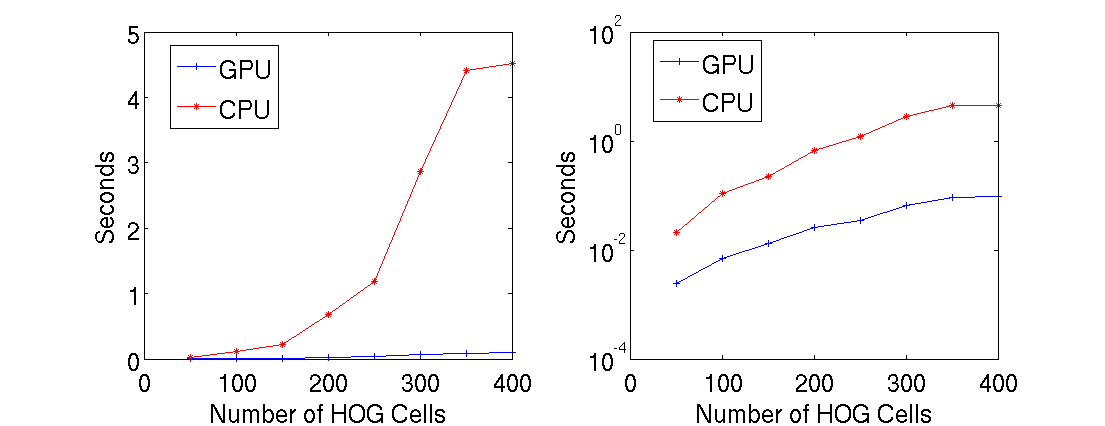
\includegraphics[width=0.9\linewidth]{covariancetime} 
  \end{center}
  \caption{Time to generate $\Sigma$ for various number of cells (left) and same plot on log scale(right). The time complexity increases as $O(n^2)$ for $n$ number of cells.}
  \label{fig:covariancetime_crop}
\end{figure}
 
% 1-dimensional version of SIMD implementation that generate covariance matrix $\Sigma$ from autocovariance $\Gamma$ on GPU is on the supplementary material.
% \begin{comment}i
% \begin{algorithm}
% \KwData{ $\Gamma$ , nonzero cell indexes, thread x id, thread y id}
% \KwResult{ $\Sigma$ }
% \Begin{
% $c_u \leftarrow \mod(x, N_f)$ define cell $u$ coordinate\; 
% $f_u \leftarrow u / N_f$ define feature index
% $c_v \leftarrow \mod(y, N_f)$ define cell $v$ coordinate\;
% $f_v \leftarrow v / N_f$ define feature index
% $T \leftarrow $ nonzero cell indexes\;
% $\Sigma(w) \leftarrow \Gamma( N_f ( T(u) - T(v) +  )$\;
% }
% \caption{SIMD implementation of covariance synthesis from autocovariance}
% \end{algorithm}
% \end{comment}

\subsection{Fast Whitening and Convolution}
\label{sec:fast_whitening}
\begin{figure}[t]
  \begin{center}
     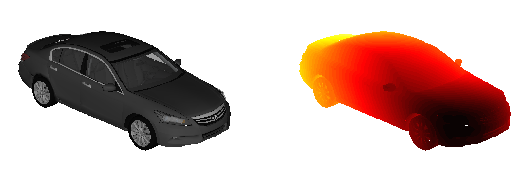
\includegraphics[width=0.9\linewidth]{whiten_orig_depth} 
  \end{center}
  \caption{Realistic rendering and depth}
  \label{fig:rendering}
  \end{figure}
 
To whiten a signal $x$, we have to solve $\Sigma w = x - \mu$. In \cite{Hariharan12}, the authors make use of the fact that covariance matrices are Hermitian and positive semidefinite to solve the system via the Cholesky decomposition, which is twice as fast as the LU decomposition. These decompositions require $O(n^3)$ time, whereas the conjugate gradient method takes $O(n^2\kappa)$ time, where $\kappa$ is the condition number of the matrix. This makes conjugate gradient a faster option for matrices with small condition numbers relative to their size.

Figure \ref{fig:spectral} shows the singular values of a covariance matrix for one HOG template after a small regularization constant is added to the diagonal. The condition number of of the matrix is \scream{x}, much smaller than the size of the matrix (7500). As a result, conjugate gradient converges in \scream{x ms}, two orders of magnitude faster than the system can be solved using the Cholesky factorization (\scream{5 s}).

The final challenge in on-the-fly template evaluation is performing the convolution between the template and the target image. Standard convolution would be prohibitively slow for the high resolution templates we're using, so we implemented the convolution via Fast Fourier Transform on the GPU. This allows template evaluation to run in \scream{x ms}, compared to \scream{x ms} for the naive CPU implementation.

  
%  If we use a high resolution template such as \ref{fig:rendering}

% where $w$ is the weight we want to find and $x$ is the HOG feature from the rendering and $\lambda$ is the regularization constant (see section \ref{sec:regularization}). For $w\in \mathcal{R}^n$, it takes $O(n^3)$ time to solve the linear equation. If we use a high resolution template to capture small geometric properties we can get high accuracy matchings but the solving the linear equation becomes computationally burdensome. 

% To briefly recap, the LU Decomposition and Cholesky Decomposition are most popular methods to solve a linear equation. In linear algebra libraries such as MATLAB, these decomposition methods are default method to solve a linear equation (backslash \textbackslash in MATLAB). Since the covariance matrix is Hermitian and Positive Semi-Definite, we can use Cholesky Decomposition which is twice as fast as the LU Decomposition.  

% decomposition methods such as LU or Cholesky Decomposition not only take long time but they also accumulate numerical error. 

%In our setting, we used high resolution template which has more than 250 HOG cells. This result in $\Sigma \in \mathcal{R}^{7500 \times 7500}$. It takes about 9 seconds if we use LU decomposition and 5 seconds if we use Cholesky decomposition.  % The default way of solving the linear equation in many linear algebra library is decomposing the matrix using LU Decomposition (in MATLAB the default method of backslash operator) which takes $O(\frac{2}{3}n^3)$ flops for $n\times n$ matrix. Since the matrix, $\Sigma + \lambda I$ is Hermitian and Positive Semi Definite. We can speed up using Cholesky Decomposition. 



%We also used iterative Conjugate Gradient to make use of low rank property of the covariance \cite{Gharbi12}. After adding small regularization, the regularized covariance matrix has nice spectral property (Figure \ref{fig:spectral}). The singular values are clustered in small region and most of the energies are concentrated on the first (number) singular values. Thus, the conjugate gradients stage doesn't go upto the size of the matrix to converge.

\begin{figure}[t]
  \begin{center}
  \begin{tabular}{cc}
     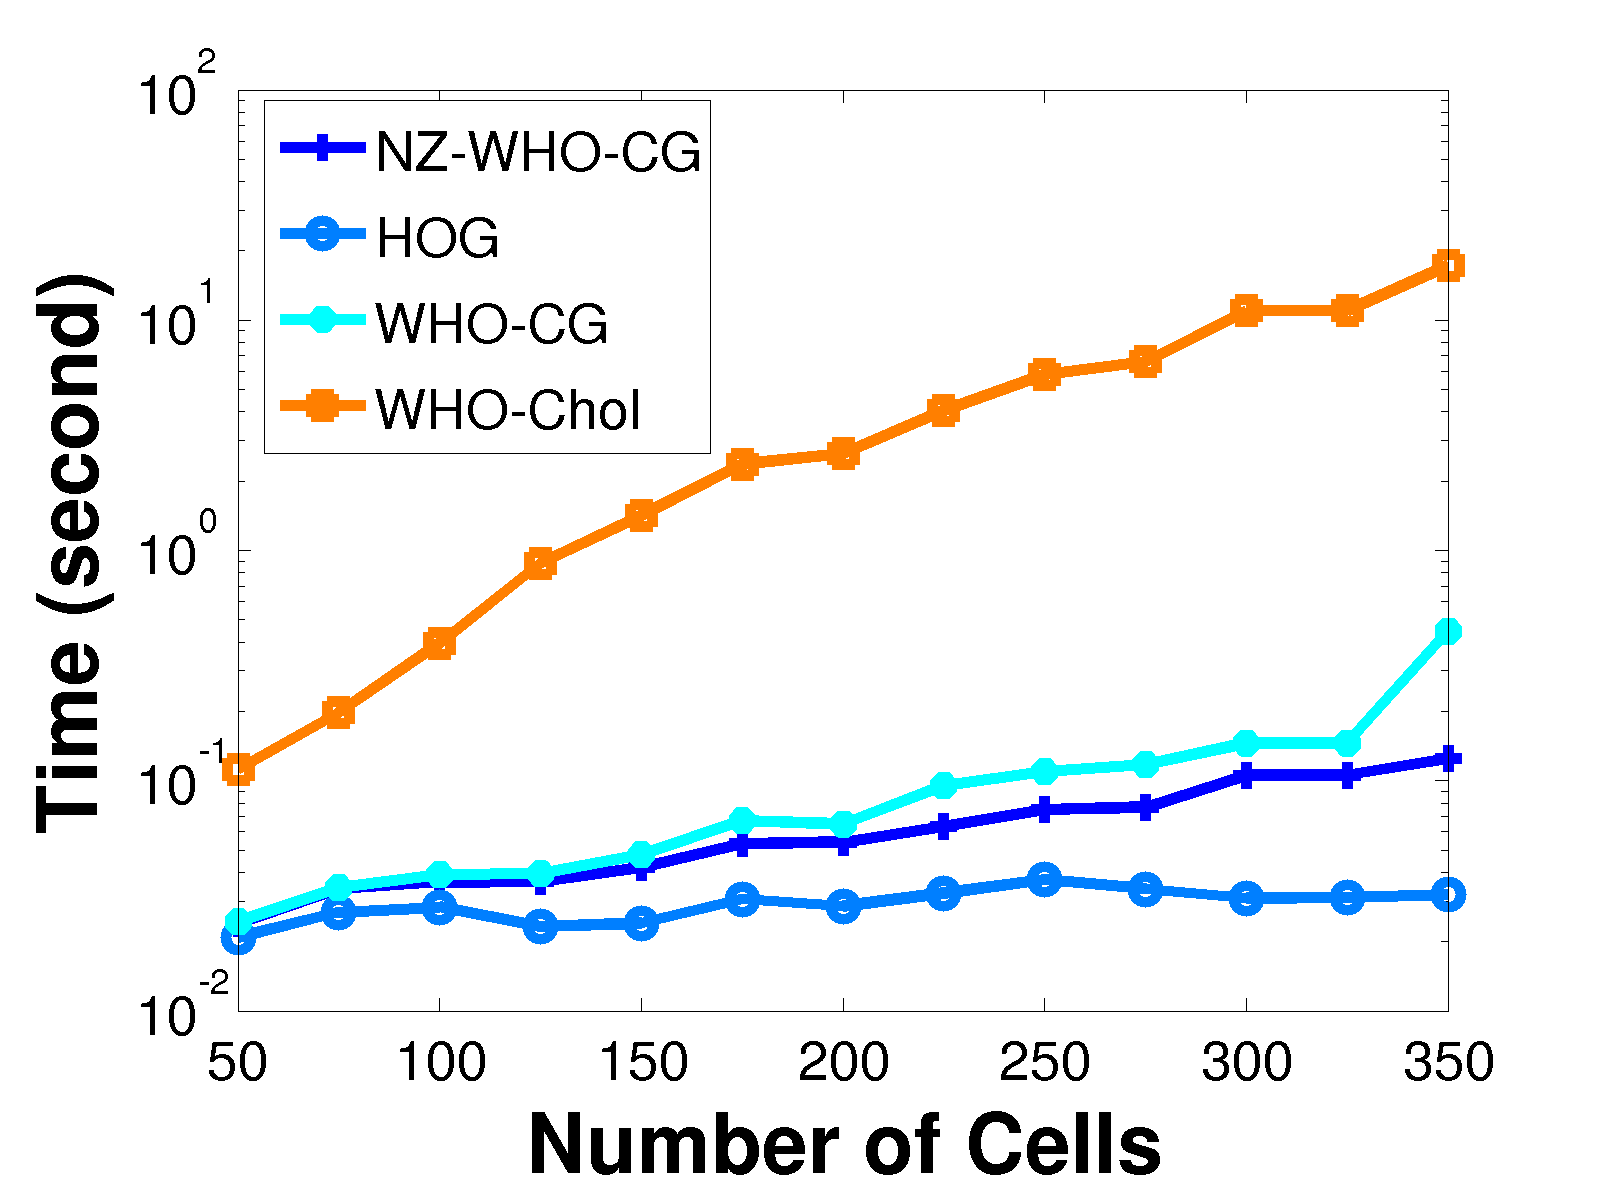
\includegraphics[width=0.5\linewidth]{whotime} & 
     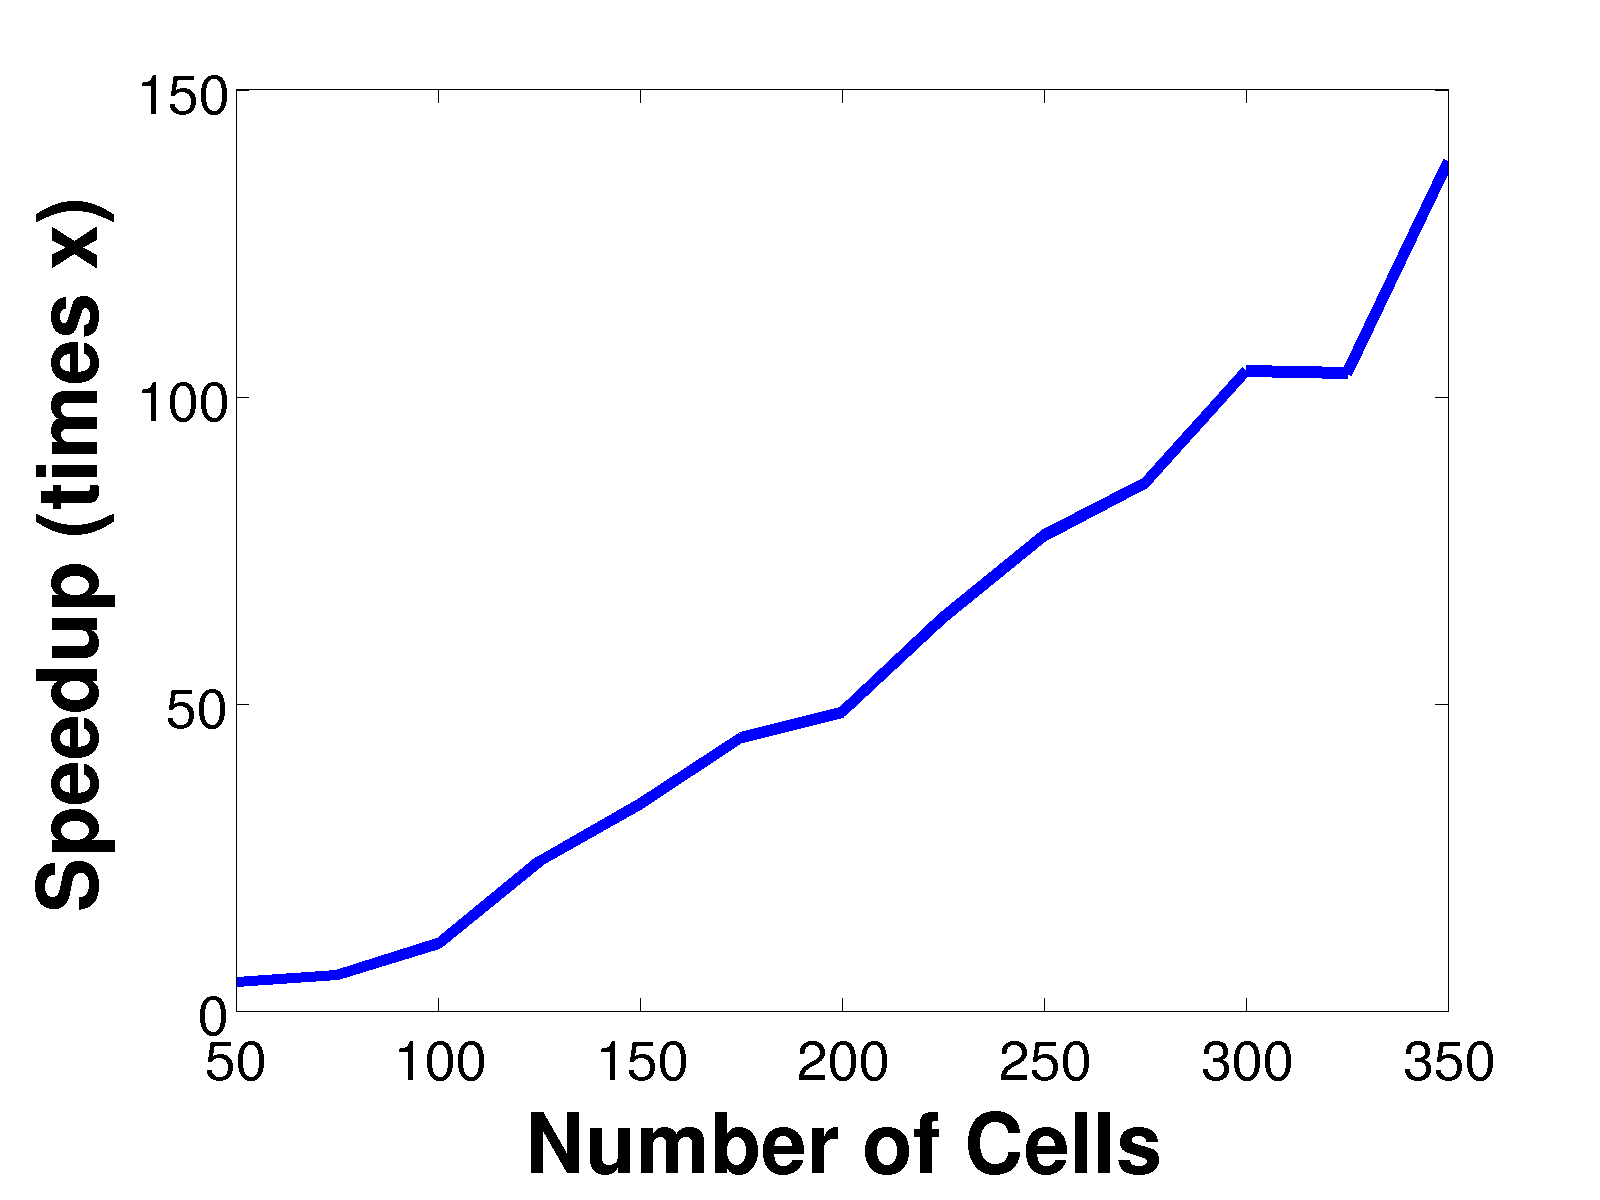
\includegraphics[width=0.5\linewidth]{speedup}\\
     (a) & (b) \\
 \end{tabular}
  \end{center}
  \caption{Comparison of HOG variants generation time and final }
  \label{fig:whotime}
\end{figure}
[Figure spectral analysis]

\begin{figure}[t]
  \centering
  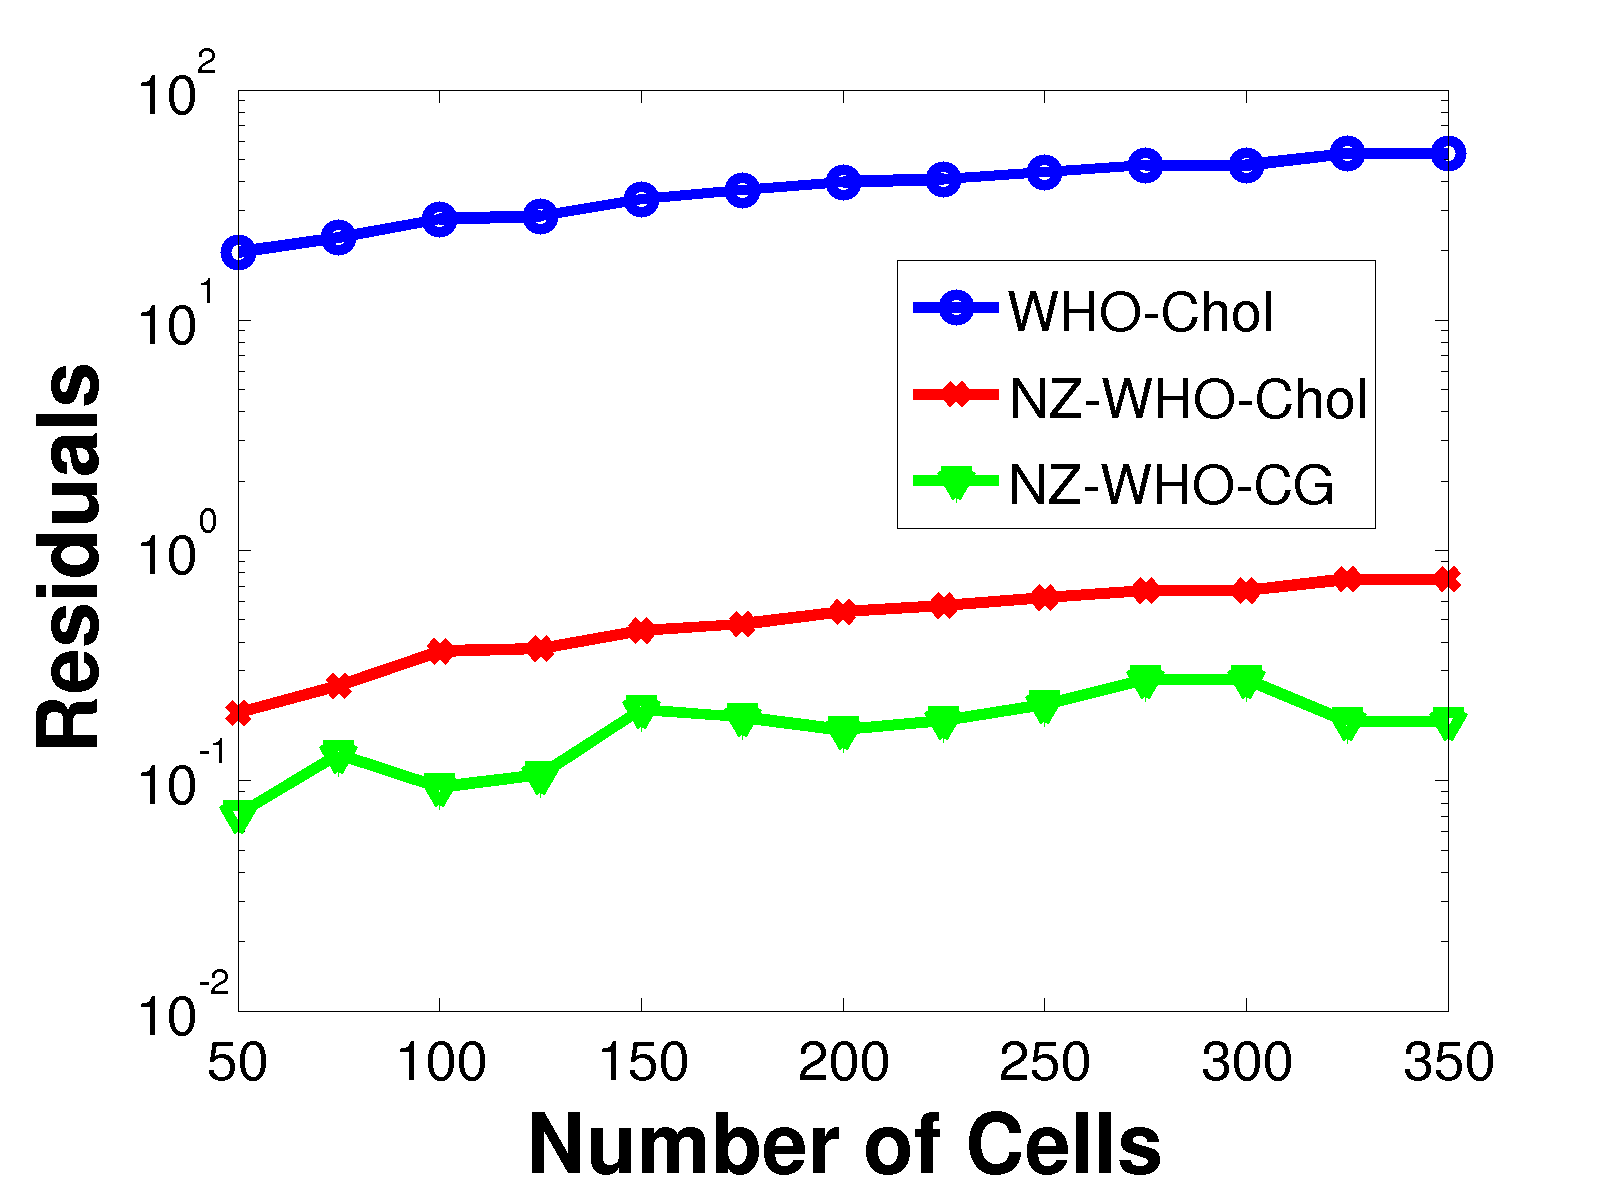
\includegraphics[width=0.5\linewidth]{residual}
  \caption{Residual of differentd method}
  \label{fig:whotime}
\end{figure}

\subsection{Variations of WHO}

We empirically found out that NZ-WHO performs reasonably well without time consuming calibration stage compare to other variational method to generate templates. We used 1 CAD model with viewpoints covering 24 azimuths and 4 elevations. Each template takes approximately 80 milliseconds to generate a NZ-WHO template. We also calibrated templates using the method presented in \cite{Aubry14}. The calibration learns affine transformation of the detection confidence.% Note that in Section \ref{experiments}, we provide the same experiment with 9 CAD models.


\begin{table*}[!htbp]
    \footnotesize
    \begin{center}
\begin{tabular}{|c|c|r|c|r|}
\hline
Methods (AP/MPPE) & before calibration  & time & after calibration \cite{Aubry14} & time \\
\hline\hline
HOG\cite{Dalal05}     & 72.3 / 65.0           &  31ms  & 60.4 / 50.2                 & 8.7 sec \\ 
WHO\cite{Hariharan12} & 82.1 / 85.4           &  3811ms& 84.4 / 83.0                 & 12.4 sec  \\
WHO-CG                & 81.7 / \textbf{84.9}  &  104ms & 83.7 / 87.3                 & 8.3 sec \\
WHO-CG-Z              & 54.4 / 65.1           &  103ms & \textbf{92.8} / 86.7        & 8.7 sec  \\
% NZC-WHO-Z    & 89.10/\textbf{78.64} &    & 91.15/74.79                  &     \\
NZ-WHO-CG             & \textbf{90.0} / 82.8  &   79ms & 90.3 / \textbf{86.8}        & 8.5 sec   \\
\hline
\end{tabular}
\end{center}
\caption{Average Precision(AP) and Mean Precision in Pose Estimation (MPPE) \cite{Lopez-Sastre11} variations of WHO on 3DObject Car dataset\cite{Savarese07}. WHO refers to standard WHO using the method presented in \cite{Hariharan12}, WHO-CG uses iterative Conjugate Gradient method to generate WHO. WHO-CG-Z uses whiten the whole template and zero out textureless region. NZ-WHO-CG is the NZ-WHO which whitens only non-zero cells using iterative Conjugate Gradient method. The time column indicates the time to generate one template. We followed calibration procedure presented in \cite{Aubry14}.}
\label{tab:who_initializations}
\end{table*}

We found out that without calibration, NZ-WHO performs the best on object detection on 3DObject car dataset \cite{Savarese07}. See Table \ref{tab:who_initializations} for detail. In essence, if we use calibration, we could achieve better performance but since our goal is to do 2D-3D matching and continuous viewpoint estimation using on-the-fly template generation, we did not calibrated our templates.


\begin{comment}
\subsection{Whitening Non-Zero Cells}

% learning weights for whitened templates
But since it is difficult to make templates to have the number of cells, \cite{Hariharan12, Aubry14, Lim14} learned weights for convolution score from the template. However, we propose a novel way to guarantee normalized score distribution by decorrelating non-zero HOG cells and forcing each template to have approximately same number of cells.

% 
Unlike \cite{Aubry14}, we did not whiten all cells and then zero out some HOG cells that are on the background. Instead, we whiten only the cells with non-zero value. We empirically found out that by whitening the cells that has non-zero support actually performs better and takes less time solving the linear equation $w = \Sigma^{-1}x$ since the number of elements to whiten decreases. However, by selecting non-zero cells, we destroys inherent Toeplitz-Block-Toeplitz property of the covariance matrix which could speed up the inversion using Fourier Transformation \cite{Akaike73, Martinsson05}.

  We propose a whitening stage for WHO feature template generation that can create template whose convolution score follow same distribution. This guarantees that we do not require any calibration stage after generating templates rapidly. We statistically compare the score distribution of whitening non-zero HOG cell only and whitening.
  \end{comment}


% \subsection{Effect of Regularization}
% \label{sec:regularization}
%  Also, since all covariance matrix is Positive Semi Definite, our matrix $\Sigma$ must be Positive Semi-Definite too. To guarantee the property, We found out that the regularization has significant impact on the performance. In \cite{Hariharan12}, Hariharan \etal used small fixed regularization since the covariance matrix of specially correlated features is intrinsically row-rank to make the matrix invertible.
%  
% However if we closely analyze the impact of the regularization, we can see that larger the $\lambda$ is, the centered HOG becomes more dominant. 
% 
% \begin{align}
% (\Sigma + \lambda I)^{-1} & = \frac{1}{\lambda}\left(I + \frac{1}{\lambda}\Sigma \right)^{-1} \\
% & = \frac{1}{\lambda}\left(I - \frac{1}{\lambda} \Sigma  + \frac{1}{\lambda^2} \Sigma^{2} 
% 		- \frac{1}{\lambda^3} \Sigma^{3} + \cdots \right)
% % & = \frac{1}{\lambda}I - \left(I + \frac{1}{\lambda} \Sigma \right)^{-1} \frac{1}{\lambda^2} \Sigma
% % & = \frac{1}{\lambda}\left(I  - \frac{1}{1 + \frac{1}{\Sigma} \Tr{\Sigma}} \right)
% \end{align} 
% 
% We empirically found out that as $\lambda$ increases, AP converges to that of centered HOG feature without any whitening.

\begin{comment}
\subsection{No Calibration}
  We created coarse viewpoint templates by whitening non-zero HOG cells and compare the average precision on 3D Object dataset \cite{Savarese07} with that of whitening all HOG cells. 
  
\begin{table}
\begin{center}
\begin{tabular}{|l|c|c|}
\hline
Whitening and AP & Whiten & No Whitening \\
\hline\hline
Average Precision & 89.205 & 74.478 \\
\hline
\end{tabular}
\end{center}
\caption{Effect of whitening on 3D Object Car validation set using one CAD model. The whitening dramatically increased the AP.}
\end{table}
\begin{table}
\begin{center}
\begin{tabular}{|l|c|c|}
\hline
Calibration methods \&AP & Whiten non-zero & Whiten all \\
\hline\hline
None & 89.205 & 86.676 \\
Linear & 88.430 & 85.720 \\
Gaussian & 87.913 & 84.567\\
Number of non-zero cells & 84.734 & N/A\\
\hline
\end{tabular}
\end{center}
\caption{Various calibration and AP on small experimental set. Since the whitening templates with constant number of HOG cells create normalized feature, calibration using negative patches did not improve the AP.}
\end{table}
\end{comment}

\begin{comment}
\subsection{High Resolution Templates and FFT based Convolution}
\label{sec:fft} 
We generate high resolution templates with more than 250 HOG cells to capture details of an object to give accurate 2D-3D matching. These large templates cause computational burden when computing convolution. Though good for detecting accurate model and pose, convolution of high-resolution templates are much more slower since computation time scales linearly with the number of HOG cells in the template. To overcome and speed up the convolution, we propose FFT based GPU convolution which scales. Suppose there are length $n$ signal and length $m$ filter, naive convolution takes $O(nm)$ time where as FFT-based convolution takes $O\left( (n + m)\log (n+m) \right)$ time. For large $m$, high resolution template, we can gain computational advantage.


we pad zero to the 2D image features by the largest kernel size. And we transform the kernel to match the padded image feature. To compute convolution, we compute element-wise product with the transformed kernel and sum all the features. Unlike \cite{Podlozhnyuk}, we do not need to shift the data nor kernel if we use simple mathematical trick. 
  
\begin{align}
    x_{pad} & = \mathcal{P}_{n+m}(x)\\
    y_{pad} & = \mathcal{P}_{n+m}(y)\\
    x_{pad} \ast y_{pad} & = \mathcal{F}^{-1}(\mathcal{F}(x_{pad}) \circ \mathcal{F}(y_{pad}))
\end{align}

  Where $\ast$ is the circular convolution and $\circ$ is the Hadamard Product and $\mathcal{F}$ is the Fourier Transformation and $\mathcal{P}_n$ is the padding operation that append zeros to make vector of size $n$.

For each dimension of features, we transform kernel and image feature into frequency domain using Fast Fourier Transformation. We transform the image into frequency domain once and use the transformed image for all templates.

We implemented the convolution using FFT on GPU and got 10x speed up.

[Figure for convolution time for different template resolution, CPU, GPU, naive convolution]
\end{comment}
%------------------------------------------------------------------------

\section{Estimating Parameters using MCMC}
\label{sec:fine}
% Estimating viewpoint continuously to fine tune a initial matching
The NZ-WHO template matching method we have presented makes template generation and evaluation computationally inexpensive. This means we can efficiently explore the parameter space to find the best object pose, scale, model type and camera focal length.



Since creating a template and validating the template become computationally inexpensive, making a proposal and validating the proposal to fine tune a 2D-3D matching became affordable. We used Metropolis-Hastings algorithm to generate a proposal pose and focal length and validate the proposal using the convolution and returning maximum response as a return.

We modeled the distribution of the convolution as an exponential distribution and used Gaussian as our proposal distribution.  

We run experiments on PASCAL 2007 car category images with at least one car (num images) and got x percent improvement after fine tuning.

% there are several advantages that was not possible such as \textbf{on-the-fly} template generation and making large number of templates  
\begin{figure}[t]
\centering
    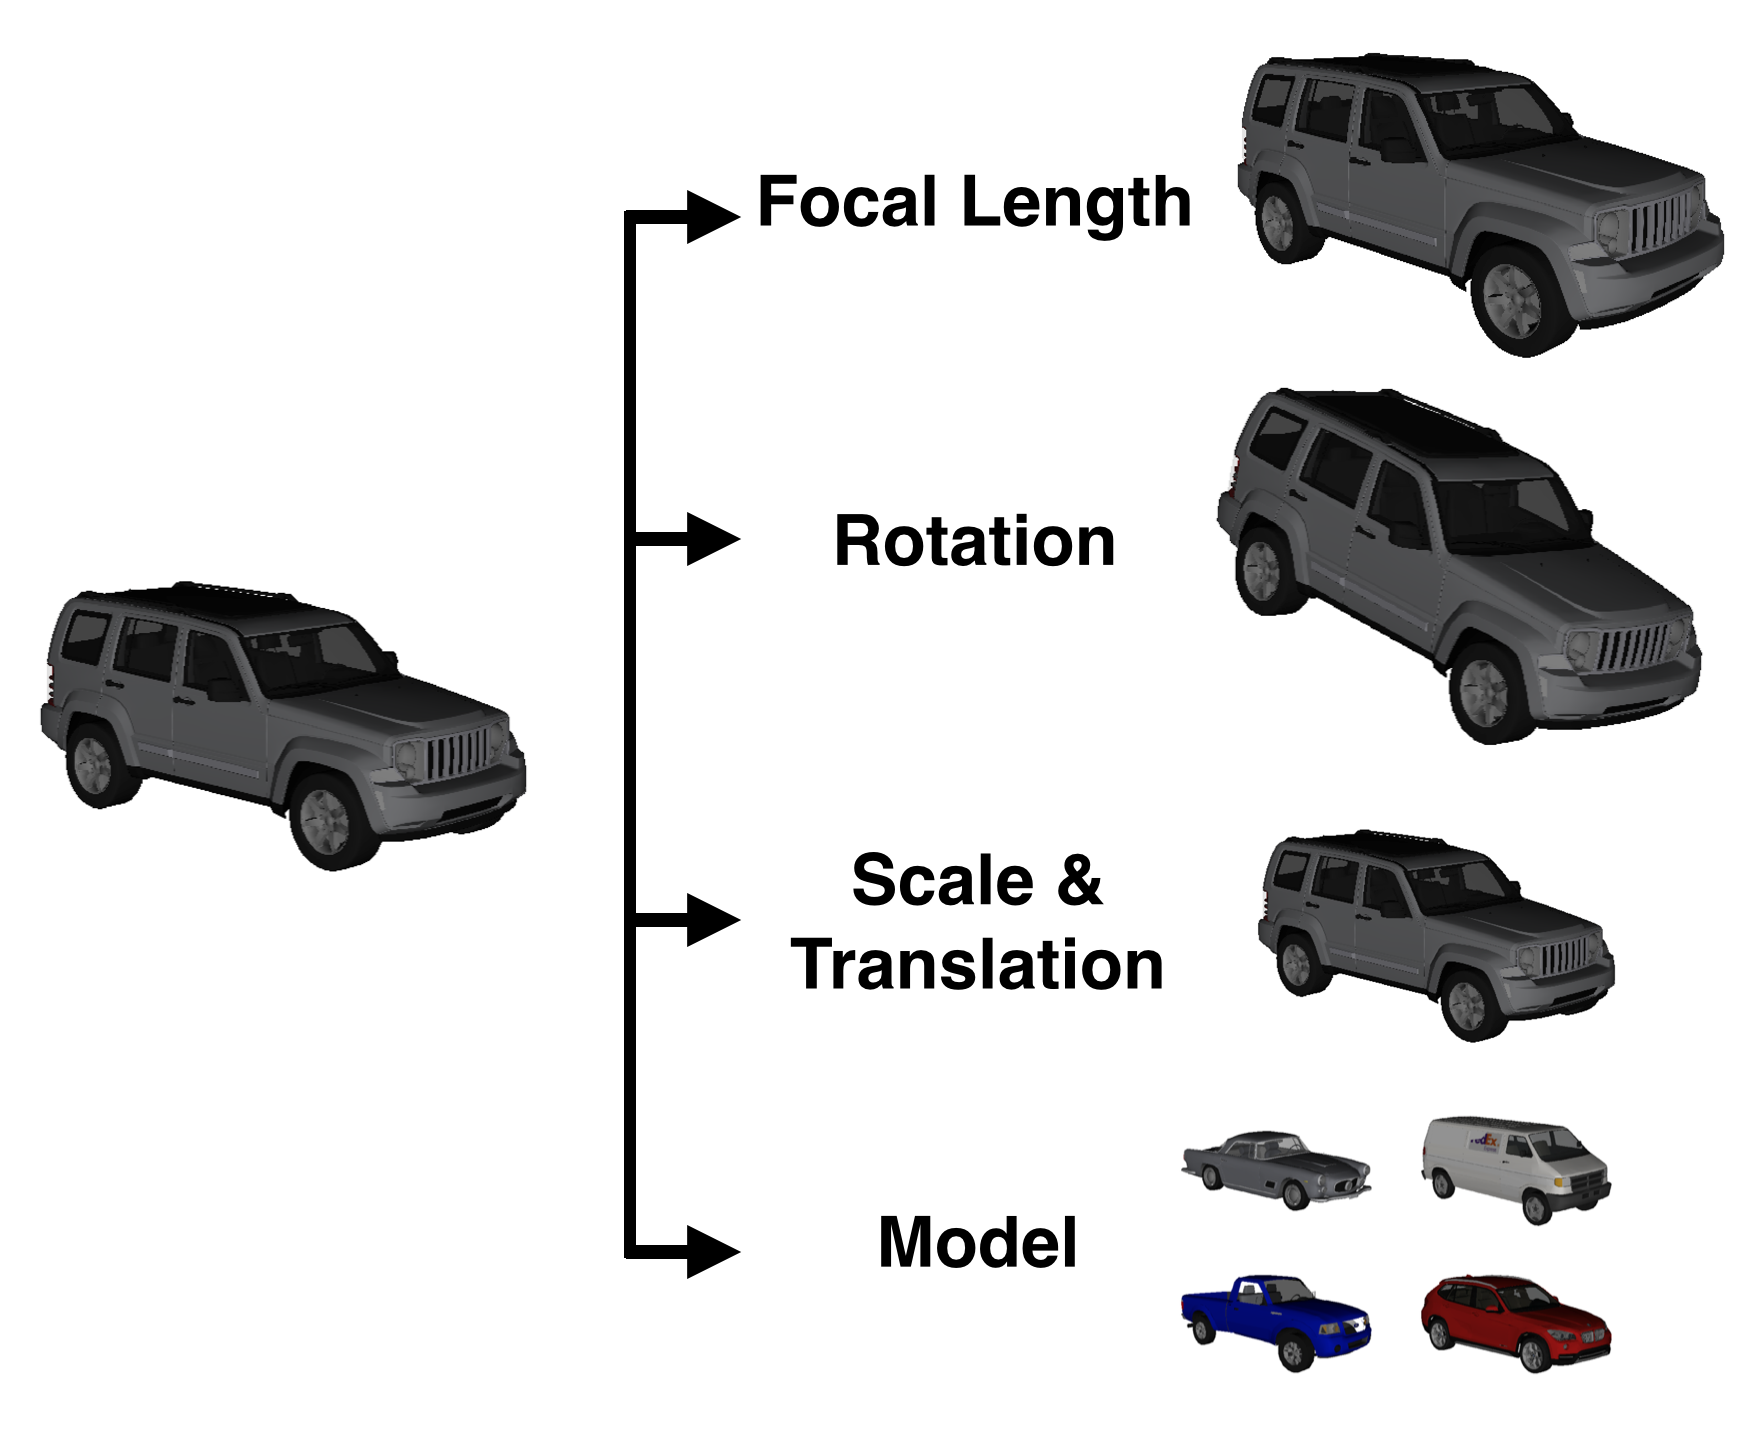
\includegraphics[width=0.7\linewidth]{tuning2} \\ [-5pt]
    \caption{Different modes of Metropolis Hasting proposals, see Section \ref{sec:fine}}
 \label{fig:tuningmode}
\end{figure}
    
\begin{figure}[t]
 \begin{center}
    \setlength\tabcolsep{0pt}
    \begin{tabular}{ccc}
    % 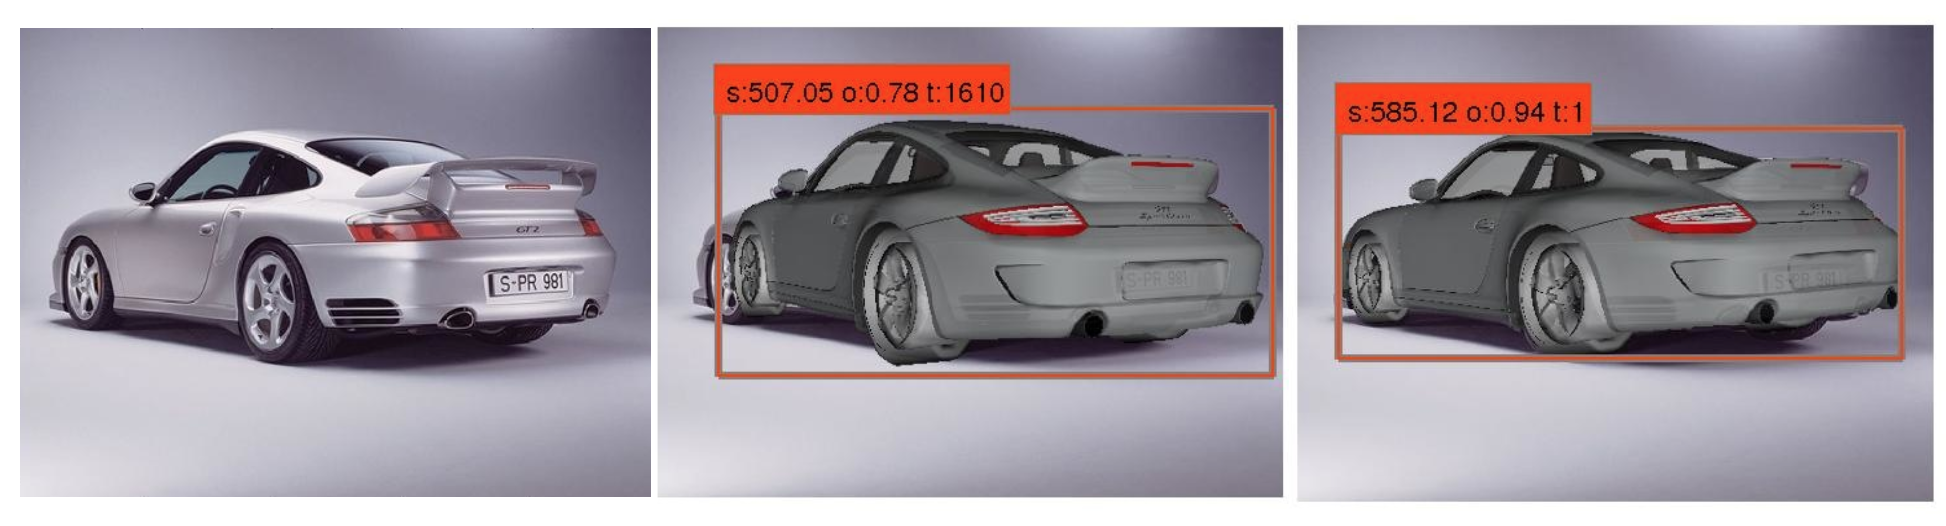
\includegraphics[width=0.9\linewidth]{tuning} 
   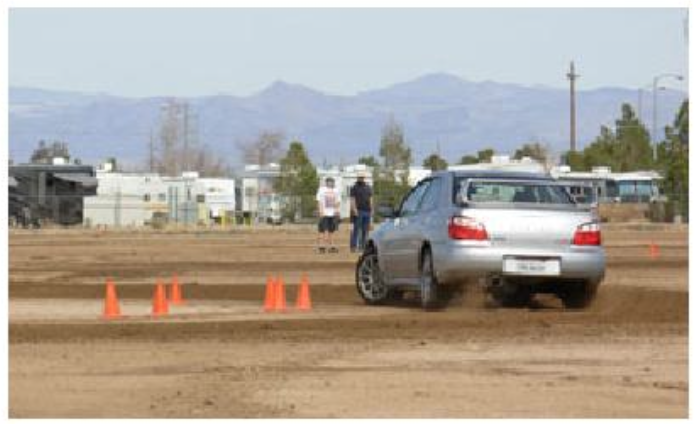
\includegraphics[width=0.33\linewidth]{tuning/1.png} &
   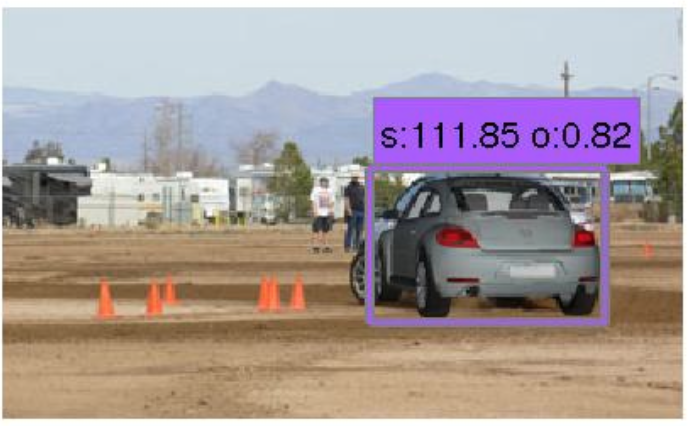
\includegraphics[width=0.33\linewidth]{tuning/2.png} &
   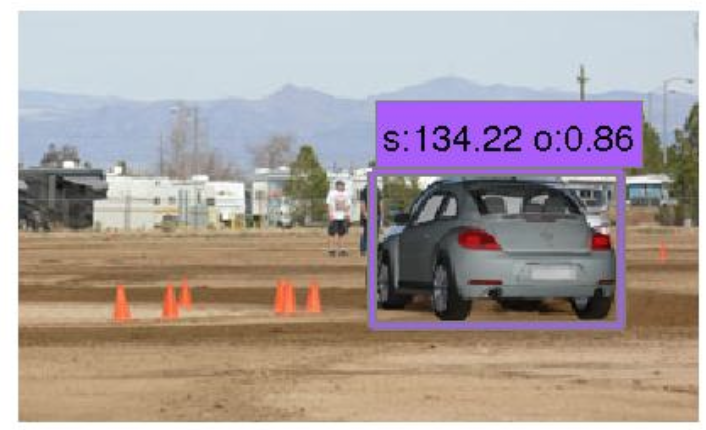
\includegraphics[width=0.33\linewidth]{tuning/3.png} \\[-5pt]
   (a) & (b) & (c)\\
   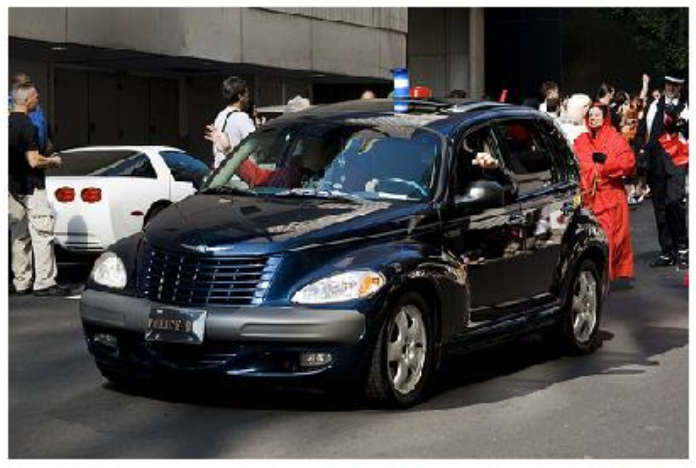
\includegraphics[width=0.33\linewidth]{tuning/4.png} &
   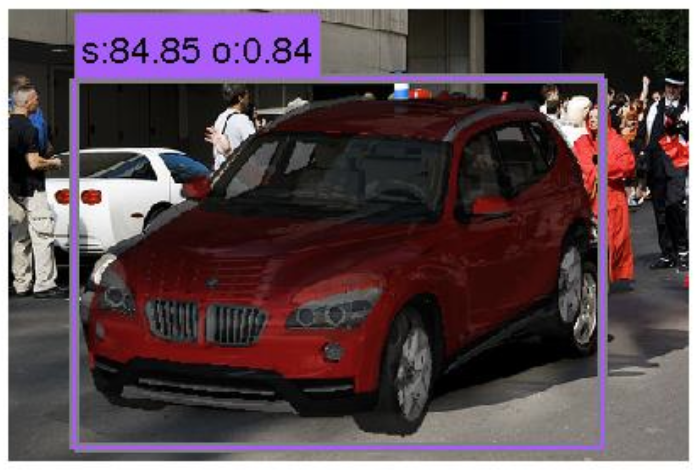
\includegraphics[width=0.33\linewidth]{tuning/5.png} &
   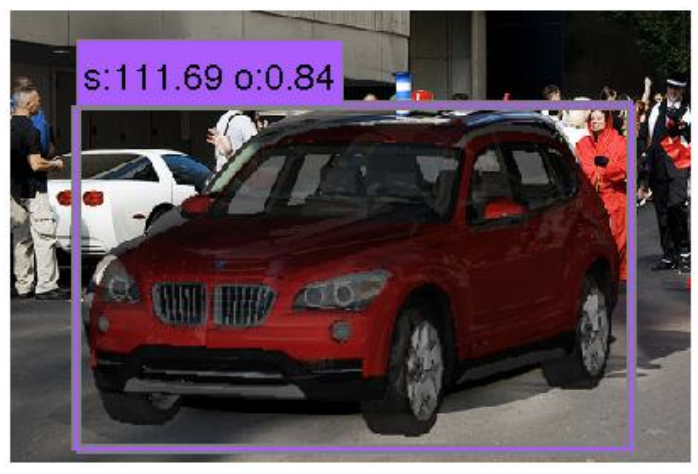
\includegraphics[width=0.33\linewidth]{tuning/6.png} \\[-5pt]
   (d) & (e) & (f)\\
   \end{tabular}
 \end{center}
 \caption{Effect of fine tuning. (left) original image, (middle) initial detection, (right) continuous fine tuning}
 \label{fig:tuning}
\end{figure}



\section{Experiments}

In this section, we validate our proposed NZ-WHO templates in two different ways. First, we make a set of NZ-WHO templates for a set of CAD models from various viewpoints. Then we run the bank of NZ-WHO templates as ensembles of weak detectors and show that the rendering image can be We want to see how robust the NZ-WHO to real images a

Second, we show that our method can complement the detection bounding boxes coming out of standard object detectors. This process will enrich object detection bounding boxes with 2D-3D matching which gives continuous viewpoint estimation, a CAD model (rendering, depth) and fine-grained category.  

\subsection{2D-3D Matching as an Object Detector} 

We created ensemble of NZ-WHO templates using 9 CAD models and measured the Average Precision (AP) of object detection task and Mean Precision in Pose Estimation (MPPE) \cite{Lopez-Sastre11}. MPPE is the average of viewpoint accuracy.  

% Instance-level 2D-3D matching (registration) is a difficult problem since we need a CAD model that looks similar to the object in the image. Especially, due to extreme intraclass variability of chair \cite{Aubry14} used a very large collection of CAD models to cover variety of chairs. Similarly, \cite{Lim14}

Our ensemble of NZ-WHO templates is generated from rendering images within few minutes but shows reasonable performance on object detection task. The baseline method are Aspect Layout Model (ALM) \cite{Xiang12} and VOC-DPM \cite{Pepik12}. Note that the baseline methods require complex 3D modeling and viewpoint annotated natural images.

The detection result is on Table \ref{tab:3dobject} and example output from our method is on Figure \ref{fig:3dobject}. 

\begin{table}[!htbp]
    \footnotesize
  \begin{center}
    \begin{tabular}{|c|c|c|c|}
    \hline
     AP/MPPE& Ours & ALM\cite{Xiang12} & VOC-DPM\cite{Pepik12} \\
    \hline\hline
    car & \textbf{99.8}/91.7 &  98.4/93.4 & \textbf{99.8}/\textbf{97.5} \\ 
    bicycle & 93.0/87.4 & 93.0/91.4 & \textbf{98.8}/\textbf{97.5} \\
    \hline
    \end{tabular}
  \end{center}
  \caption{Average Precision(AP) and Mean Precision in Pose Estimation (MPPE) on 3DObject dataset car category. Our method produces high quality 2D-3D matching yet performs on par with state-of-the art detectors.}
  \label{tab:3dobject}
\end{table}

\begin{figure}[h]
    \begin{center}
    \setlength\tabcolsep{0pt}
\begin{tabular}{cc}
  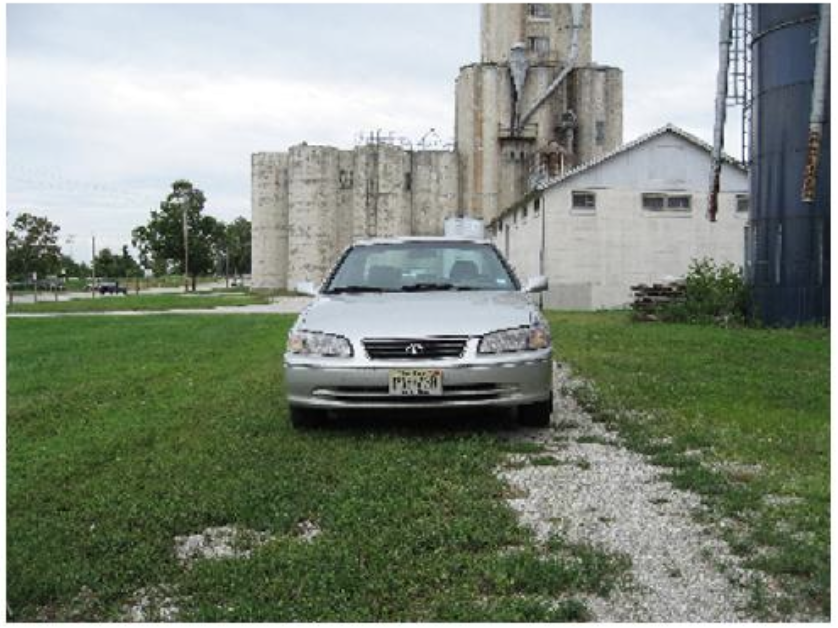
\includegraphics[width=0.45\linewidth]{car_3dobject/7.png} &   
  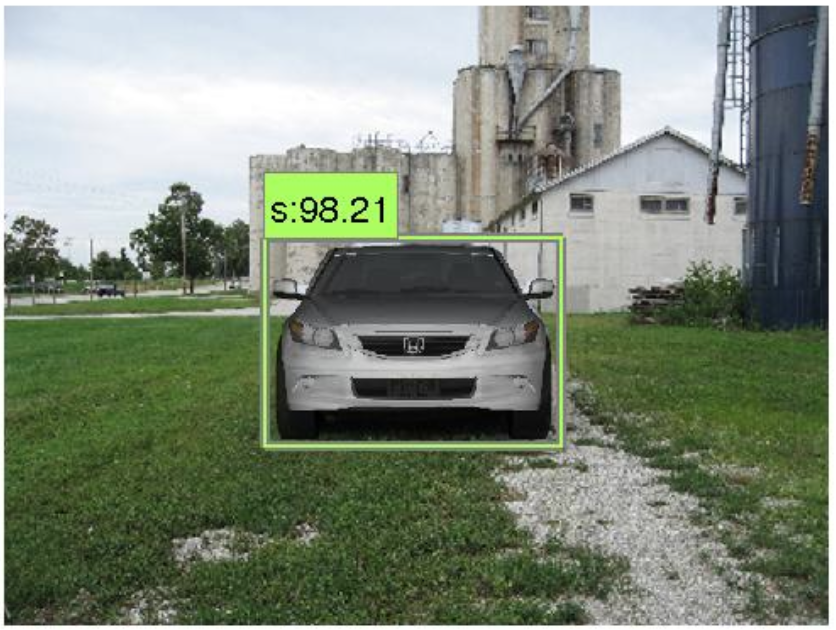
\includegraphics[width=0.45\linewidth]{car_3dobject/8.png}\\ [-15pt]
%   (a) & (b) \\[0pt]
  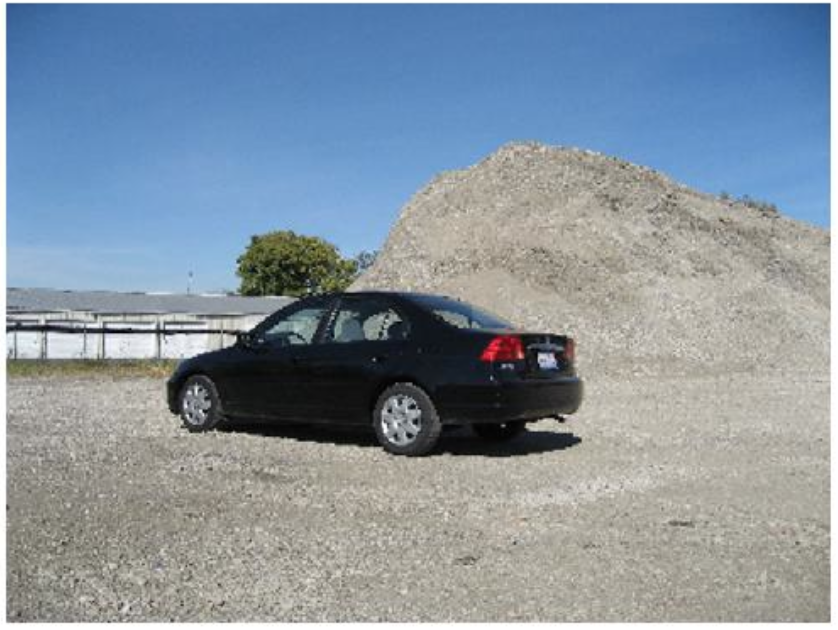
\includegraphics[width=0.45\linewidth]{car_3dobject/11.png} &   
  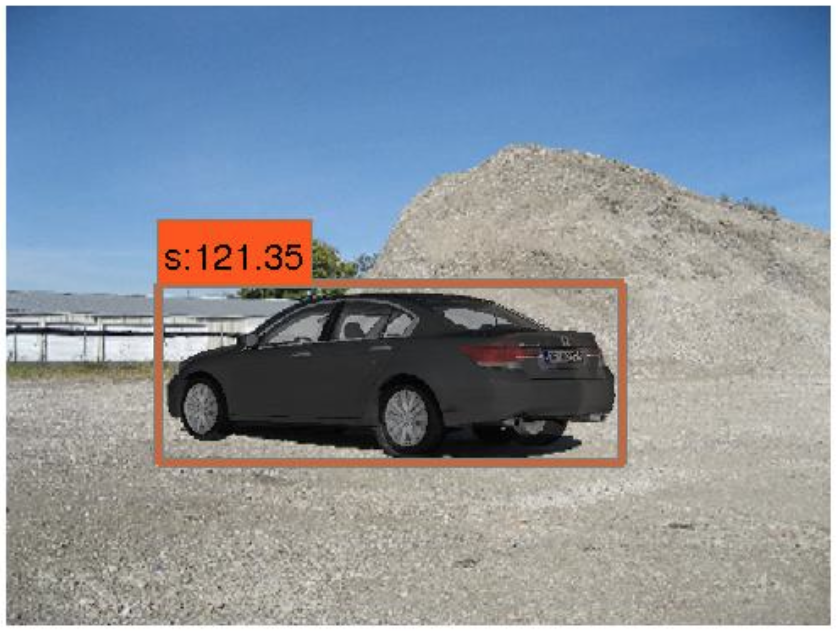
\includegraphics[width=0.45\linewidth]{car_3dobject/12.png}\\ [-5pt]
%  (c) & (d) \\[0pt]
\end{tabular}
\end{center}
\caption{Detection results on 3D-Object dataset \cite{Savarese07}. Original image (left) and detection result overlaid on top with a bounding box and corresponding confidence score(right)}
  \label{fig:3dobject}
\end{figure}


% Also, we evaluated our method on PASCAL 2007 dataset.
% 
% \begin{table}[!htbp]
%   \begin{center}
%   \begin{tabular}{|c|c|c|c|c|}
%     \hline
%      AP &    Ours &    ELDA \cite{Hariharan12} & ESVM \cite{Malisiewicz11} & VOCDPM \cite{Pepik12} \\
%     \hline\hline
%     car      & 27.          &  38.4  & 40.1    &65.7  \\ 
%     bicycle  & 43.74 & 41      &  40.7   & 61.3   \\
%     \hline
%     \end{tabular}
%   \end{center}
%   \caption{Average Precision(AP) on PASCAL 2007 dataset. Though we do not need any training images and made templates in few minues, it performs on par with state of the art detector yet it gives high quality 2D-3D matching.}
%   \label{tab:pascal07}
% \end{table}

\subsection{Fine-Tuning and Viewpoint Estimation}

High performance object detectors usually generalizes very well. It can handle various intraclass variability, viewpoint change and occlusion. However due to this high generalization, sometimes it is very difficult to get accurate pose, category or 2D-3D matching. Our method, specialized in giving such accurate information, can be applied on any generic object detectors to give high quality metadata.

To show such ability, we evaluated our method on PASCAL 3D dataset \cite{Xiang14}. The dataset augments PASCAL 2012 images with high quality viewpoint annotations thus is ideal to measure pose estimation. The dataset proposes new metric called Average Viewpoint Precision (AVP) where it measures the area under viewpoint precision and detection recall curve. The viewpoints is measured by azimuth similarity. If the distance between predicted azimuth and ground truth azimuth is below a certain threshold, the viewpoint is correct. Note that the baseline methods (V-DPM, VOC-DPM) reported on the PASCAL 3D dataset are variants of DPM where each component of DPM account for various azimuths. Thus V-DPM and VOC-DPM provide discrete azimuth only whereas our method provides 3D viewpoint (yaw, pitch, roll), CAD instance (model index, rendering, depth) and focal length.

We used detection bounding boxes and augment it using our method to give viewpoint estimation. We used detection bounding boxes from two different methods: VOC-DPM \cite{Pepik12} and R-CNN \cite{Girshick14}. VOC-DPM is a variation of DPM that can estimate viewpoint and is the state-of-the-art performance in viewpoint estimation \cite{Xiang14}. The result is on Table \ref{tab:pascal12} and precision recall curves for car using R-CNN + Ours are on Figure \ref{fig:car_cnn_ap}. 

We got significant improvement on viewpoint estimation by using our method on top of general purpose detectors. Note that our method estimates azimuth, elevation, in-plane rotation, focal length estimation, fine-grained categorization whereas V-DPM, VOC-DPM only estimate discrete viewpoints.

Example outputs are on Figure \ref{fig:pascal12cnn}.


\begin{figure*}[h]
\setlength\tabcolsep{1pt}
\centering
\begin{tabular}{|c|c|c|c|c|}
   \hline
  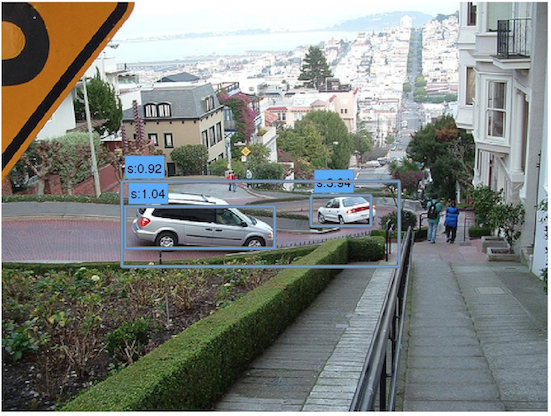
\includegraphics[width=0.24\textwidth]{car_cnn/1a.png} &   
  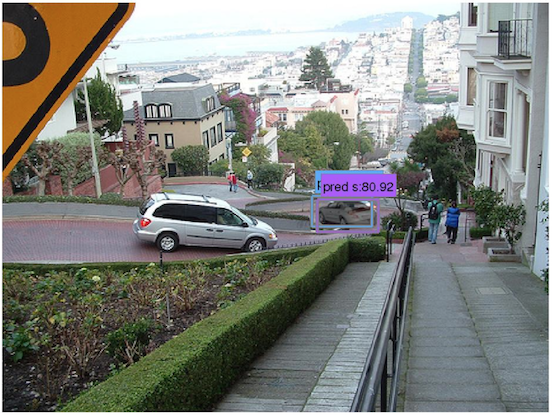
\includegraphics[width=0.24\textwidth]{car_cnn/1b.png} &   
  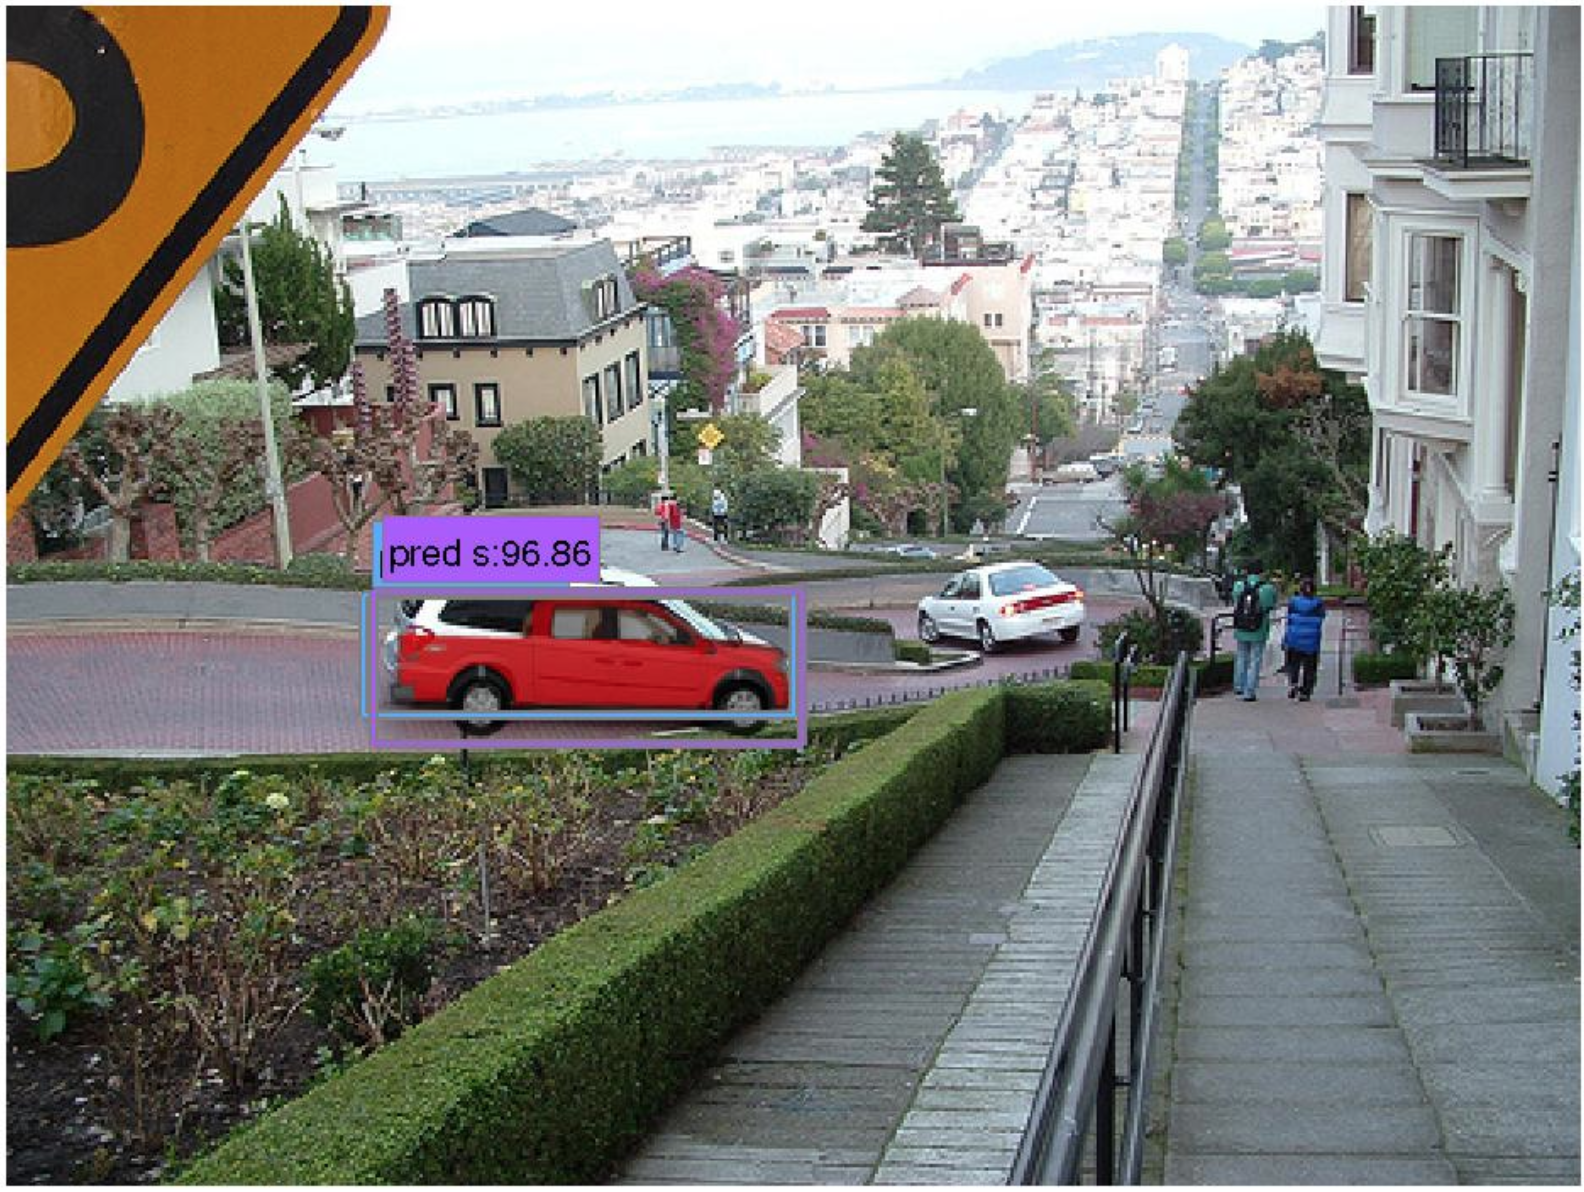
\includegraphics[width=0.24\textwidth]{car_cnn/1c.png} &   
  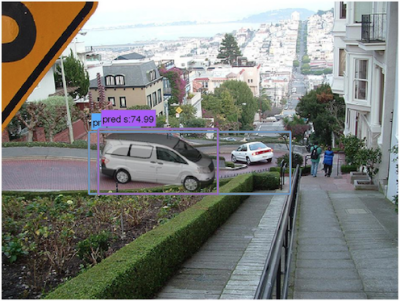
\includegraphics[width=0.24\textwidth]{car_cnn/1d.png}  \\  
   \hline
  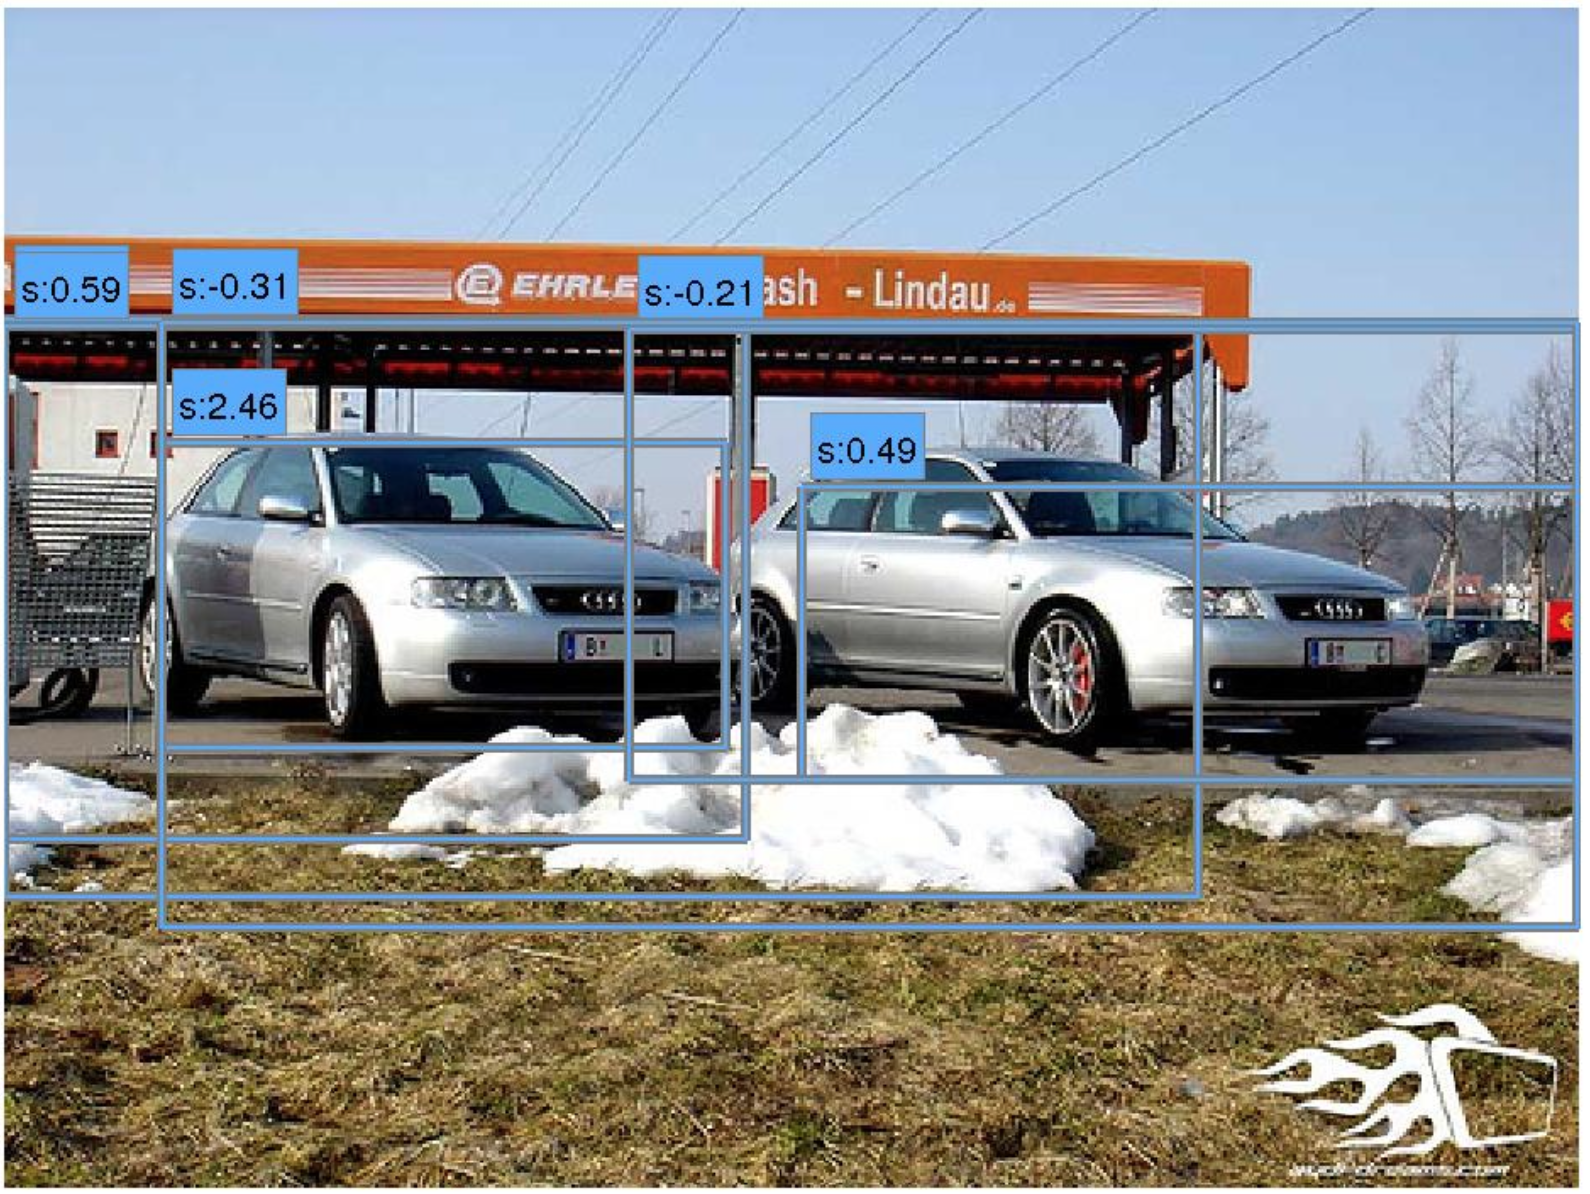
\includegraphics[width=0.24\textwidth]{car_cnn/2a.png} &   
  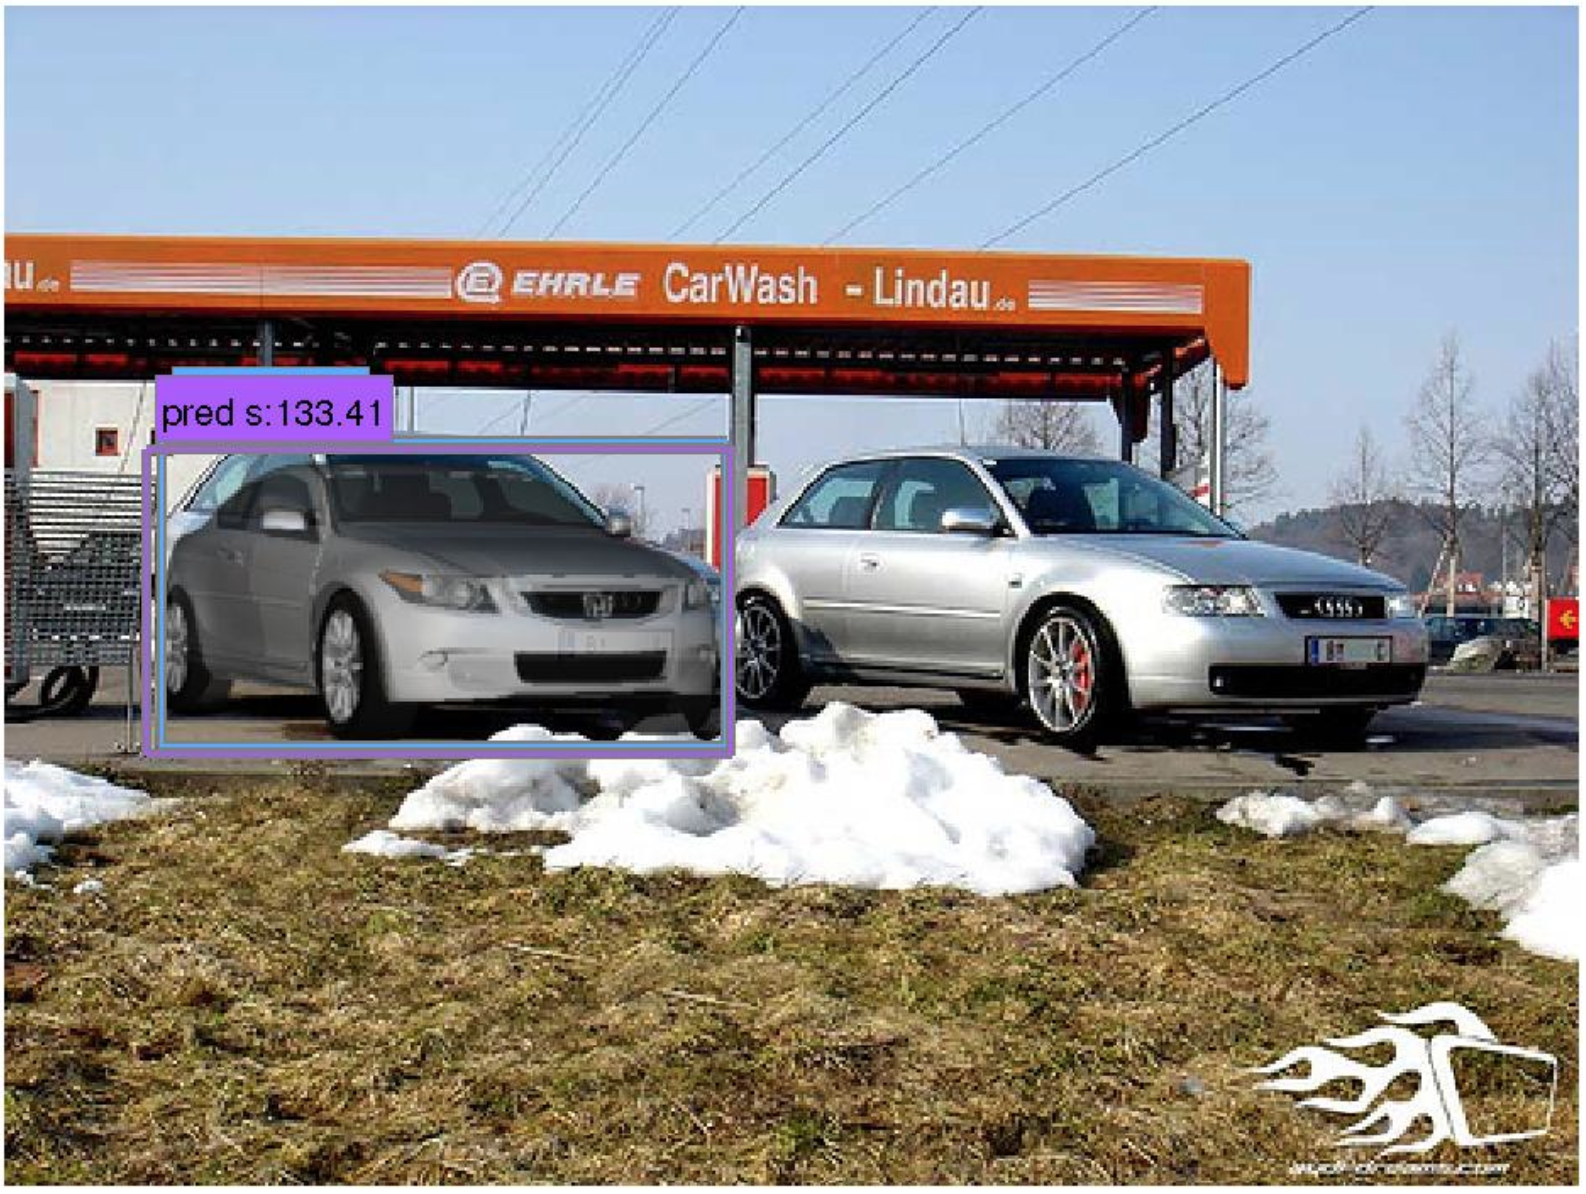
\includegraphics[width=0.24\textwidth]{car_cnn/2b.png} &   
  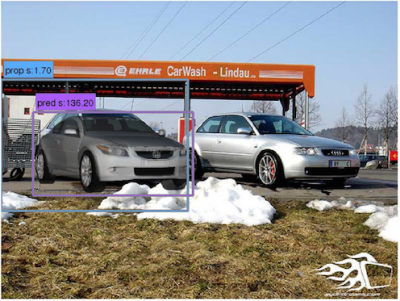
\includegraphics[width=0.24\textwidth]{car_cnn/2c.png} &   
  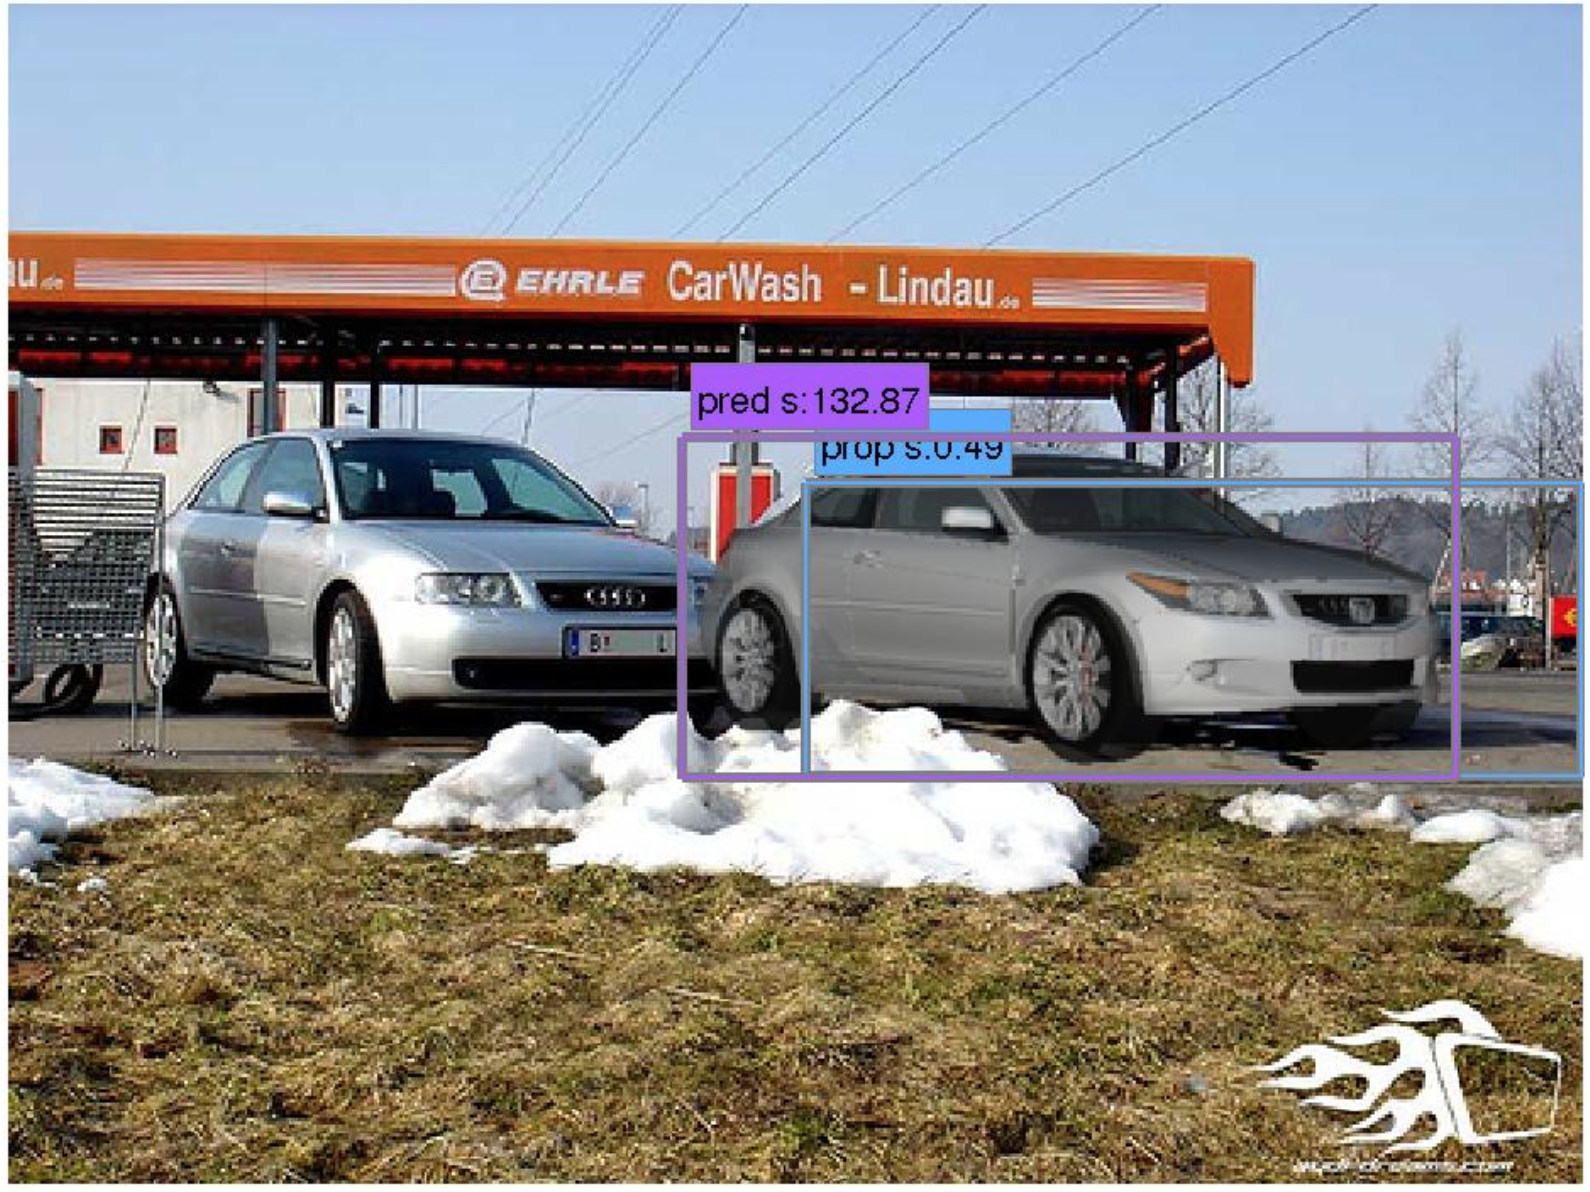
\includegraphics[width=0.24\textwidth]{car_cnn/2e.png}  \\  
   \hline
  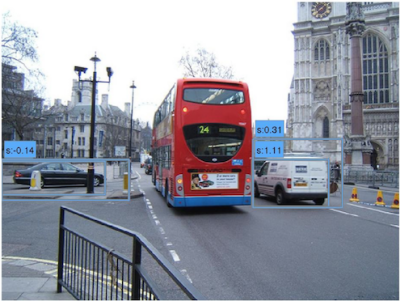
\includegraphics[width=0.24\textwidth]{car_cnn/4a.png} &   
  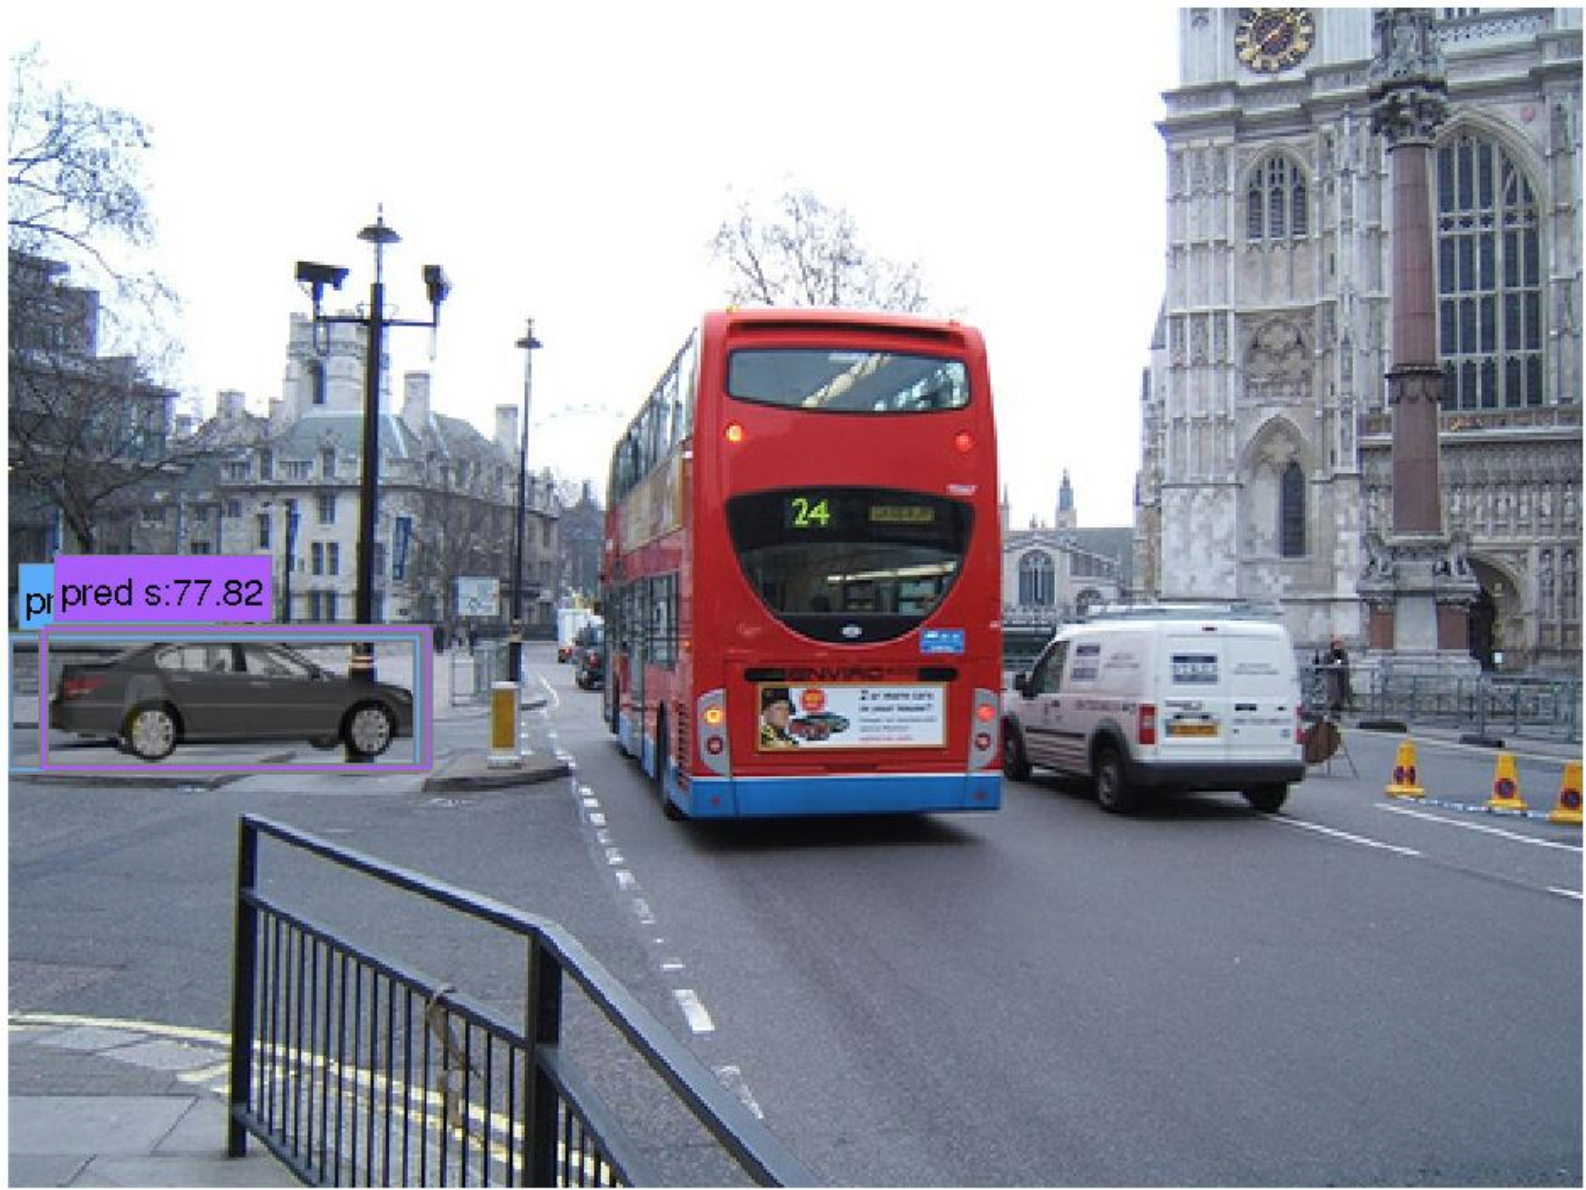
\includegraphics[width=0.24\textwidth]{car_cnn/4b.png} &   
  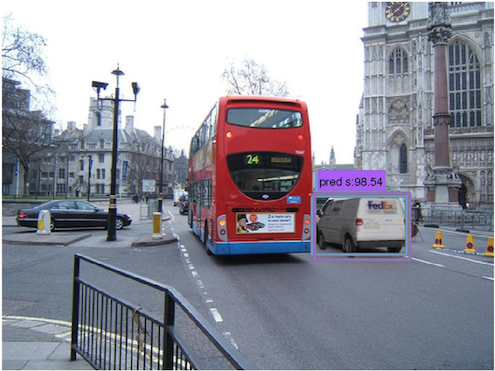
\includegraphics[width=0.24\textwidth]{car_cnn/4c.png} &   
  \includegraphics[width=0.24\textwidth]{car_cnn/4d.png}  \\  
%    \hline
%   \includegraphics[width=0.24\textwidth]{car_cnn/10a.png} &   
%   \includegraphics[width=0.24\textwidth]{car_cnn/10b.png} &   
%   \includegraphics[width=0.24\textwidth]{car_cnn/10c.png} &   
%   \includegraphics[width=0.24\textwidth]{car_cnn/10d.png}  \\  
%   \hline 
%   \includegraphics[width=0.24\textwidth]{bicycle_cnn/3a.png} &   
%   \includegraphics[width=0.24\textwidth]{bicycle_cnn/3b.png} &   
%   \includegraphics[width=0.24\textwidth]{bicycle_cnn/3c.png} &   
%   \includegraphics[width=0.24\textwidth]{bicycle_cnn/3d.png}  \\
  \hline
  \includegraphics[width=0.24\textwidth]{bicycle_cnn/7a.png} &   
  \includegraphics[width=0.24\textwidth]{bicycle_cnn/7b.png} &   
  &\\
  \hline
  \includegraphics[width=0.24\textwidth]{bicycle_cnn/4a.png} &   
  \includegraphics[width=0.24\textwidth]{bicycle_cnn/4b.png} &   
  \includegraphics[width=0.24\textwidth]{bicycle_cnn/4c.png} &   
  \includegraphics[width=0.24\textwidth]{bicycle_cnn/4d.png}  \\
  \hline
  CNN Proposals & \multicolumn{3}{|c|}{Our matching results on proposal bounding boxes} \\
  \hline
\end{tabular}
\caption{Example enriched bounding boxes. Given R-CNN\cite{Girshick14} detection bounding boxes, our method predicted 2D-3D matching reasonably. On the first column, R-CNN detection bounding boxes overlaid. From the second to the last columns, output of our method given a R-CNN box. Blue boxes are R-CNN output and purple boxes are the tightest bounding box enclosing predicted CAD model}
  \label{fig:pascal12cnn}
\end{figure*}
\begin{table*}[!htbp]
    \footnotesize
  \begin{center}
\begin{tabular}{|c|c|c|c|c|c|c|}
\hline
AP/AVP              & V-DPM \cite{Xiang14} & VOC-DPM \cite{Pepik12}  & \cite{Pepik12} + Ours (discrete) & \cite{Pepik12} + Ours (full) & R-CNN + Ours (discrete) & R-CNN + Ours (full)\\
\hline\hline
car-4v              & 37.2 / 20.2         & 45.6 / 36.9             & 47.6 / 42.7       & 47.6 / \textbf{42.7}        & 49.6 / 41.5         & 49.6 / 41.5\\ \hline
car-8v              & 37.3 / 23.5         & 47.6 / 36.6             & 47.6 / \textbf{39.8}       & 47.6 / 39.5        & 49.6 / 38.0         & 49.6 / 39.0\\ \hline
car-16v             & 36.6 / 18.1         & 46.0 / 29.6             & 47.6 / 32.7       & 47.6 / 33.0        & 49.6 / 34.0         & 49.6 / \textbf{34.3}\\ \hline
car-24v             & 36.3 / 13.7         & 42.1 / 24.6             & 47.6 / 27.4       & 47.6 / 27.4        & 49.6 / 27.0         & 49.6 / \textbf{27.6}\\ \hline
\hline
bicycle-4v          & 45.2 / 41.7         & 46.9 / 43.9             & 48.1 / 47.6       & 48.1 / 46.6        & 61.7 / 56.5         & 61.7 / \textbf{56.7}\\ \hline
bicycle-8v          & 47.3 / 36.7         & 48.1 / 40.3             & 48.1 / 40.6       & 48.1 / 40.6        & 61.7 / 48.9         & 61.7 / \textbf{49.2}\\ \hline
bicycle-16v         & 46.5 / 18.4         & 45.6 / 22.9             & 48.1 / 26.2       & 40.1 / 27.3        & 61.7 / 34.7         & 61.7 / \textbf{35.8}\\ \hline
bicycle-24v         & 44.4 / 14.3         & 45.9 / 16.7             & 48.1 / 21.5       & 40.1 / 20.9        & 61.7 / \textbf{27.0}         & 61.7 / 23.9\\ \hline
\end{tabular}
\end{center}
\caption{Average Precision(AP) and Average Viewpoint Precision(AVP) on PASCAL 3D dataset\cite{Xiang14}. For combined method (* + Ours), we use bounding boxes from * and augment viewpoint using our method. R-CNN and run our method to produce 2D-3D matching. If our method fails to give viewpoint, it predicts the viewpoint to be 0. Note that our method gives high quality metadata such as continuous 3D viewpoint, CAD model (rendering depth) and fine-grained category, whereas base-line methods gives 1D discrete azimuths. Our R-CNN was not an optimized version so the detection AP is lower than the state-of-the-art R-CNN performance}
\label{tab:pascal12}
\end{table*}

\begin{figure}[h]
\setlength\tabcolsep{1pt}
\centering
\begin{tabular}{cc}
  \hline
  \includegraphics[width=0.49\linewidth]{car_cnn4_crop.png} &   
  \includegraphics[width=0.49\linewidth]{car_cnn8_crop.png} \\   
  \includegraphics[width=0.49\linewidth]{car_cnn16_crop.png} &   
  \includegraphics[width=0.49\linewidth]{car_cnn24_crop.png} \\   
  \hline
\end{tabular}
\caption{Average Precision (AP) and Average Viewpoint Precision (AVP) and viewpoint confusion table on PASCAL 12 car validation set using R-CNN + Ours. From the top left, 4 views, 8 views, 16 views and 24 views. Since our method only augment the object detection, the AP remains the same for all cases. As we increase the viewpoint estimation, the AVP decreases. Note that since we estimate null viewpoint if our method fails to find match, there are more 0 viewpoint predictions (top row of confusion matrices) }
  \label{fig:car_cnn_ap}
\end{figure}

\subsection{Stability of Our Method for Irregular Bounding Boxes}

% Generic object detectors give overlapping detection bounding boxes of the same object which can be handled by non maximal suppression. For these overlapping detections, 

R-CNN detection bounding boxes are irregular in shape since they come from other region proposal methods and sometimes they truncate objects. To handle such irregular shape and truncation, we added small context around the bounding boxes and run our method. 

We assumed that object can be arbitrarily truncated by the bounding box and search all plausible scales and translations. This can be efficiently computed using FFT-based convolution (refer Section. \ref{sec:fft}). We put examples of such conditions in Figure \ref{fig:stability}. Although the input bounding boxes are irregular and truncate objects, our method reliably generated a reasonable prediction of pose, translation, scale and CAD model.



\begin{figure}[h]
\setlength\tabcolsep{5pt}
\begin{tabular}{cc}
  \includegraphics[width=0.45\linewidth]{car_pascal/1.png} &   
  \includegraphics[width=0.45\linewidth]{car_pascal/2.png} \\   
  \includegraphics[width=0.45\linewidth]{car_pascal/3.png} &   
  \includegraphics[width=0.45\linewidth]{car_pascal/4.png} \\   
\end{tabular}
\caption{Stability of our method for overlapping R-CNN detection \cite{Girshick14}. Blue box is the R-CNN detection that is feed into the system as initial detection. Purple box and overlaid rendering is the final output of the system. Note that for various overlapping bounding boxes, our system accurately estimated the reasonable result}
  \label{fig:stability}
\end{figure}


% For qualitative examples, we put hand-picked results from our method Fig. \ref{fig:car} and Fig. \ref{fig:bicycle}.

% \begin{figure*}[h]
% \setlength\tabcolsep{5pt}
% \begin{tabular}{|c|c|c|}
%     \hline
%   \includegraphics[width=0.325\textwidth]{car/PASCAL_car_val_init_0_Car_each_27_lim_250_lam_0_150_a_24_e_3_y_1_f_1_scale_2_00_sbin_6_level_15_skp_n_server_101_img_39.jpg} &   
%   \includegraphics[width=0.325\textwidth]{car/PASCAL_car_val_init_0_Car_each_27_lim_250_lam_0_150_a_24_e_3_y_1_f_1_scale_2_00_sbin_6_level_15_skp_n_server_101_img_78.jpg} & 
%   \includegraphics[width=0.325\textwidth]{car/PASCAL_car_val_init_0_Car_each_27_lim_250_lam_0_150_a_24_e_3_y_1_f_1_scale_2_00_sbin_6_level_15_skp_n_server_101_img_85.jpg} \\[-15pt]
% (a) & (b) & (c) \\[0pt]
% \hline
%   \includegraphics[width=0.325\textwidth]{car/PASCAL_car_val_init_0_Car_each_27_lim_250_lam_0_150_a_24_e_3_y_1_f_1_scale_2_00_sbin_6_level_15_skp_n_server_101_img_338.jpg} &   
%   \includegraphics[width=0.325\textwidth]{car/PASCAL_car_val_init_0_Car_each_27_lim_250_lam_0_150_a_24_e_3_y_1_f_1_scale_2_00_sbin_6_level_15_skp_n_server_101_img_360.jpg} & 
%   \includegraphics[width=0.325\textwidth]{car/PASCAL_car_val_init_0_Car_each_27_lim_250_lam_0_150_a_24_e_3_y_1_f_1_scale_2_00_sbin_6_level_15_skp_n_server_101_img_414.jpg} \\[-15pt]
% (d) & (e) & (f) \\[0pt]
% \hline
%   \includegraphics[width=0.325\textwidth]{car/PASCAL_car_val_init_0_Car_each_27_lim_250_lam_0_150_a_24_e_3_y_1_f_1_scale_2_00_sbin_6_level_15_skp_n_server_101_img_418.jpg} &   
%   \includegraphics[width=0.325\textwidth]{car/PASCAL_car_val_init_0_Car_each_27_lim_250_lam_0_150_a_24_e_3_y_1_f_1_scale_2_00_sbin_6_level_15_skp_n_server_101_img_1049.jpg} & 
%   \includegraphics[width=0.325\textwidth]{car/PASCAL_car_val_init_0_Car_each_27_lim_250_lam_0_150_a_24_e_3_y_1_f_1_scale_2_00_sbin_6_level_15_skp_n_server_101_img_1242.jpg} \\[-15pt]
% (g) & (h) & (i) \\[0pt]
% \hline
%   \includegraphics[width=0.325\textwidth]{car/PASCAL_car_val_init_0_Car_each_27_lim_250_lam_0_150_a_24_e_3_y_1_f_1_scale_2_00_sbin_6_level_15_skp_n_server_101_img_1244.jpg} &   
%   \includegraphics[width=0.325\textwidth]{car/PASCAL_car_val_init_0_Car_each_27_lim_250_lam_0_150_a_24_e_3_y_1_f_1_scale_2_00_sbin_6_level_15_skp_n_server_101_img_1261.jpg} & 
%   \includegraphics[width=0.325\textwidth]{car/PASCAL_car_val_init_0_Car_each_27_lim_250_lam_0_150_a_24_e_3_y_1_f_1_scale_2_00_sbin_6_level_15_skp_n_server_101_img_1452.jpg} \\[-15pt]
% (j) & (k) & (l) \\[0pt]
% \hline
%   \includegraphics[width=0.325\textwidth]{car/PASCAL_car_val_init_0_Car_each_27_lim_250_lam_0_150_a_24_e_3_y_1_f_1_scale_2_00_sbin_6_level_15_skp_n_server_101_img_1467.jpg} &   
%   \includegraphics[width=0.325\textwidth]{car/PASCAL_car_val_init_0_Car_each_27_lim_250_lam_0_150_a_24_e_3_y_1_f_1_scale_2_00_sbin_6_level_15_skp_n_server_101_img_1553.jpg} & 
%   \includegraphics[width=0.325\textwidth]{car/PASCAL_car_val_init_0_Car_each_27_lim_250_lam_0_150_a_24_e_3_y_1_f_1_scale_2_00_sbin_6_level_15_skp_n_server_101_img_1597.jpg} \\[-15pt]
% (m) & (n) & (o) \\[3pt]
% \hline
% \end{tabular}
%   \caption{Selected detections from PASCAL 07 Car categories. From the left, (1) original image, (2) overlaid true positive CAD models, (3) overlaid true positive CAD models with bounding boxes, (4) overlaid false positive CAD models with bounding boxes. Bounding box is colored from red (high confidence) to blue (low confidence) }
%   \label{fig:car}
% \end{figure*}
% \begin{figure*}[h]
% \setlength\tabcolsep{5pt}
% \begin{tabular}{|c|c|c|}
%     \hline
%   \includegraphics[width=0.325\textwidth]{bicycle/PASCAL_bicycle_val_init_0_Bicycle_each_4_lim_250_lam_0_150_a_48_e_4_y_5_f_1_scale_2_00_sbin_6_level_15_skp_n_server_102_img_459.jpg} &   
%   \includegraphics[width=0.325\textwidth]{bicycle/PASCAL_bicycle_val_init_0_Bicycle_each_4_lim_250_lam_0_150_a_48_e_4_y_5_f_1_scale_2_00_sbin_6_level_15_skp_n_server_102_img_1300.jpg} &   
%   \includegraphics[width=0.325\textwidth]{bicycle/PASCAL_bicycle_val_init_0_Bicycle_each_4_lim_250_lam_0_150_a_48_e_4_y_5_f_1_scale_2_00_sbin_6_level_15_skp_n_server_102_img_539.jpg} \\[-15pt]
% (a) & (b) & (c) \\[0pt]
% \hline
%   \includegraphics[width=0.325\textwidth]{bicycle/PASCAL_bicycle_val_init_0_Bicycle_each_4_lim_250_lam_0_150_a_48_e_4_y_5_f_1_scale_2_00_sbin_6_level_15_skp_n_server_102_img_35.jpg} &   
%   \includegraphics[width=0.325\textwidth]{bicycle/PASCAL_bicycle_val_init_0_Bicycle_each_4_lim_250_lam_0_150_a_48_e_4_y_5_f_1_scale_2_00_sbin_6_level_15_skp_n_server_102_img_83.jpg} &   
%   \includegraphics[width=0.325\textwidth]{bicycle/PASCAL_bicycle_val_init_0_Bicycle_each_4_lim_250_lam_0_150_a_48_e_4_y_5_f_1_scale_2_00_sbin_6_level_15_skp_n_server_102_img_131.jpg} \\[-15pt]
% (d) & (e) & (f) \\[0pt]
% \hline
%   \includegraphics[width=0.325\textwidth]{bicycle/PASCAL_bicycle_val_init_0_Bicycle_each_4_lim_250_lam_0_150_a_48_e_4_y_5_f_1_scale_2_00_sbin_6_level_15_skp_n_server_102_img_175.jpg} &   
%   \includegraphics[width=0.325\textwidth]{bicycle/PASCAL_bicycle_val_init_0_Bicycle_each_4_lim_250_lam_0_150_a_48_e_4_y_5_f_1_scale_2_00_sbin_6_level_15_skp_n_server_102_img_210.jpg} &   
%   \includegraphics[width=0.325\textwidth]{bicycle/PASCAL_bicycle_val_init_0_Bicycle_each_4_lim_250_lam_0_150_a_48_e_4_y_5_f_1_scale_2_00_sbin_6_level_15_skp_n_server_102_img_233.jpg} \\[-15pt]
% (g) & (h) & (i) \\[0pt]
% \hline
%   \includegraphics[width=0.325\textwidth]{bicycle/PASCAL_bicycle_val_init_0_Bicycle_each_4_lim_250_lam_0_150_a_48_e_4_y_5_f_1_scale_2_00_sbin_6_level_15_skp_n_server_102_img_322.jpg} &   
%   \includegraphics[width=0.325\textwidth]{bicycle/PASCAL_bicycle_val_init_0_Bicycle_each_4_lim_250_lam_0_150_a_48_e_4_y_5_f_1_scale_2_00_sbin_6_level_15_skp_n_server_102_img_348.jpg} &   
%   \includegraphics[width=0.325\textwidth]{bicycle/PASCAL_bicycle_val_init_0_Bicycle_each_4_lim_250_lam_0_150_a_48_e_4_y_5_f_1_scale_2_00_sbin_6_level_15_skp_n_server_102_img_375.jpg} \\[-15pt]
% (j) & (k) & (l) \\[0pt]
% \hline
%   \includegraphics[width=0.325\textwidth]{bicycle/PASCAL_bicycle_val_init_0_Bicycle_each_4_lim_250_lam_0_150_a_48_e_4_y_5_f_1_scale_2_00_sbin_6_level_15_skp_n_server_102_img_400.jpg} &   
%   \includegraphics[width=0.325\textwidth]{bicycle/PASCAL_bicycle_val_init_0_Bicycle_each_4_lim_250_lam_0_150_a_48_e_4_y_5_f_1_scale_2_00_sbin_6_level_15_skp_n_server_102_img_434.jpg} &   
%   \includegraphics[width=0.325\textwidth]{bicycle/PASCAL_bicycle_val_init_0_Bicycle_each_4_lim_250_lam_0_150_a_48_e_4_y_5_f_1_scale_2_00_sbin_6_level_15_skp_n_server_102_img_459.jpg} \\[-15pt]
% (m) & (n) & (o) \\[3pt]
% \hline
% \end{tabular}
%   \caption{Selected detections from PASCAL 12 Bike categories. From the left, (1) original image, (2) overlaid true positive CAD models, (3) overlaid true positive CAD models with bounding boxes, (4) overlaid false positive CAD models with bounding boxes. Bounding box is colored from red (high confidence) to blue (low confidence) }
%   \label{fig:bicycle}
% \end{figure*}


% \section{Object Detection with various Training Data}
% \section{Image Query}

\section{Conclusion}


{\small
\bibliographystyle{ieee}
\bibliography{egbib}
}

\end{document}
